%!TEX root = main.tex

%% ------------------------------------------------------------------------- %%
\chapter{Experimentos computacionais}
\label{cap:experimentos}
Neste capítulo apresentamos os resultados de experimentos computacionais
 realizados para comparar as duas formulações lineares
inteiras que propusemos no Capítulo~\ref{cap:mwstp} para o \textit{problema
  da árvore $t$-spanner de peso mínimo} (MWTSP). Também apresentamos
os resultados computacionais relativos à implementação do
algoritmo de \emph{branch-and-price} para o \textit{problema de
  $t$-spanner de peso mínimo} (MWSP).

Conforme discutimos na Seção~\ref{sec:gc_mwtsp} do capítulo anterior,
a implementação do algoritmo de \emph{branch-and-price} para o MWSP
pode ser usada para o MWTSP. Realizamos testes computacionais para
comparar esta implementação com o desempenho das formulações inteiras
propostas para o MWTSP.

\section{Ambiente computacional e programas}
Para realizar os experimentos computacionais, utilizamos o pacote de
\emph{software} de otimização CPLEX~\cite{Cplex2018}, versão~12.5,
configurado para utilizar uma única \emph{thread} do
processador. Para a implementação do algoritmo de \emph{branch-and-price},
desabilitamos o pré-processamento do CPLEX em decorrência
da geração de colunas, como sugere o manual do resolvedor.  Os
algoritmos foram implementados utilizando a linguagem de programação
C++. O código foi executado num computador com 65~GB de memória RAM e
processador de 1.6~GHz.  Para implementar alguns algoritmos
tradicionais para problemas de grafos, utilizamos a biblioteca
\emph{Lemon}~\cite{Lemon2016}.  Para gerar as instâncias de entrada
utilizamos o \emph{software} Scilab~\cite{Scilab2018}.

\section{Configuração dos parâmetros}
\label{sec:parametros}
Utilizamos como base dos nossos experimentos o trabalho de Sigurd e
Zachariasen~\cite{SigurdZ2004}, para escolher certos parâmetros e
valores. Adicionalmente, introduzimos novos parâmetros e valores aos
nossos experimentos. 

Nos experimentos realizados, variamos seis parâmetros:

\begin{itemize}
\item \emph{Ordem do grafo}: número de vértices.
  Variamos entre 16 e 100 vértices.
\item \emph{Densidade}: percentagem de arestas existentes no grafo de
  entrada, quando comparado ao grafo completo de mesma ordem.
  Consideramos densidades de 20\% a 100\%;
\item \emph{Tipo do grafo}: tipo do grafo com relação ao peso de suas
  arestas.  Consideramos grafos com pesos unitários, com distância
  euclidiana, e pesos aleatórios.  No caso de distância euclidiana,
  consideramos que os vértices do grafo estão espalhados no
  $\espacoRdois$, dentro de um quadrado de lado $100$. No caso dos
  grafos com pesos aleatórios, temos dois casos:
  \begin{itemize}
  \item valores mais espaçados: pesos pertencentes ao conjunto
    $\{1, 2, 4, 8, 16\}$, cada qual com a mesma probabilidade de ser escolhido;
  \item valores menos espaçados: pesos pertencentes ao conjunto 
    $\{1, 2, 3\}$, cada qual com a mesma probabilidade de ser escolhido;   
  \end{itemize}
\sisetup{round-mode=places,round-precision=1}  
\item \emph{Fator de dilatação}: consideramos os valores $\num{1,1}$; $2$; $3$; e $4$;
\sisetup{round-mode=places,round-precision=0}
\item \emph{Grau médio dos vértices}: utilizamos os valores 4 e 8;
\item \emph{Tempo limite}: para cada instância consideramos os tempos
  limite de execução de 1800 e 3600 segundos (de CPU). 
\end{itemize}

A construção dos nossos grafos é feita de tal forma que as arestas são
adicionadas de maneira aleatória, onde a probabilidade de adioná-las é
a mesma, respeitando as restrições que são impostas para cada
instância. Por exemplo, para um grafo de densidade de $x$\%, para cada
par de vértices $u$, $v$, a probabilidade de a aresta $uv$ ser
inserida no grafo é de $x$\%.

Nos experimentos feitos, para cada combinação de parâmetros em que o
limite de tempo é 1800~segundos, criamos 20~instâncias (reservamos 1800s
para cada instância). Em decorrência
da quantidade de experimentos realizados, para cada combinação em que
o limite de tempo é 3600 segundos, criamos 10 instâncias
(novamente, reservamos 3600s para cada instância). Os valores
indicados de tempo referem-se à
média considerando-se as instâncias resolvidas (a ser explicado a seguir)
dentre o grupo de 20 (resp. 10) instâncias.  O tempo médio foi arrendondado
para o inteiro mais próximo. Com relação à
implementação do algoritmo de \emph{branch-and-price}, alguns testes
mostraram que vale a pena adotar o critério (a) (veja
Seção~\ref{sec:estrategia_ramificacao}) como forma de escolher a
variável fracionária para fazer a ramificação. Os dados exibidos neste
capítulo foram obtidos com esse critério.

Consideramos que uma instância é resolvida quando, dentro do limite de
tempo estabelecido, a implementação encontra uma solução ótima ou verifica
que não existe uma solução viável (para o caso de árvores
$t$-spanner).

A heurística (veja Seção~\ref{sec:mwsp_preprocessamento}) apresentada 
para as formulações lineares inteiras para o MWTSP (para o caso unitário)
não foi executada nestes experimentos para que pudéssemos medir e
comparar o desempenho das formulações lineares inteiras.

\section{Resultados para árvore $t$-spanner de peso mínimo}
\begin{figure}[t]%
    \centering
    \subfloat{{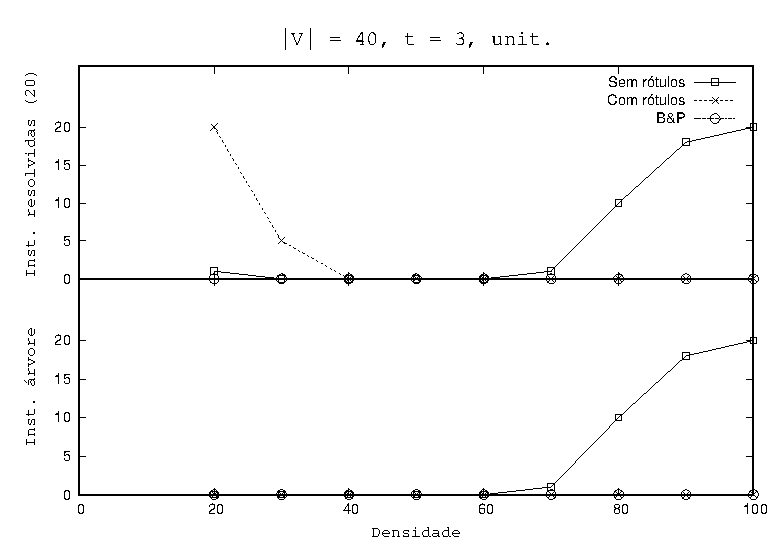
\includegraphics[scale=0.60]{figuras/2inst_den-sf3-s40-unit} }}%
    %\;
    \subfloat{{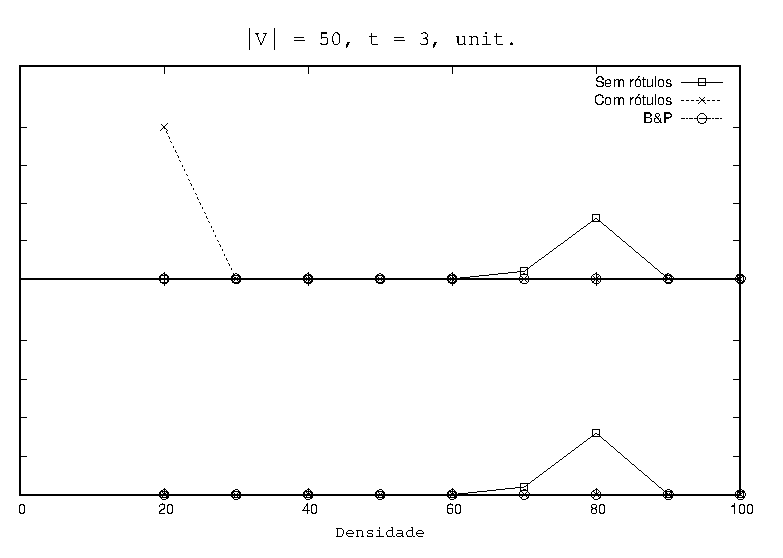
\includegraphics[scale=0.60]{figuras/2inst_den-sf3-s50-unit} }}    
    %% \subfloat[label 2]{{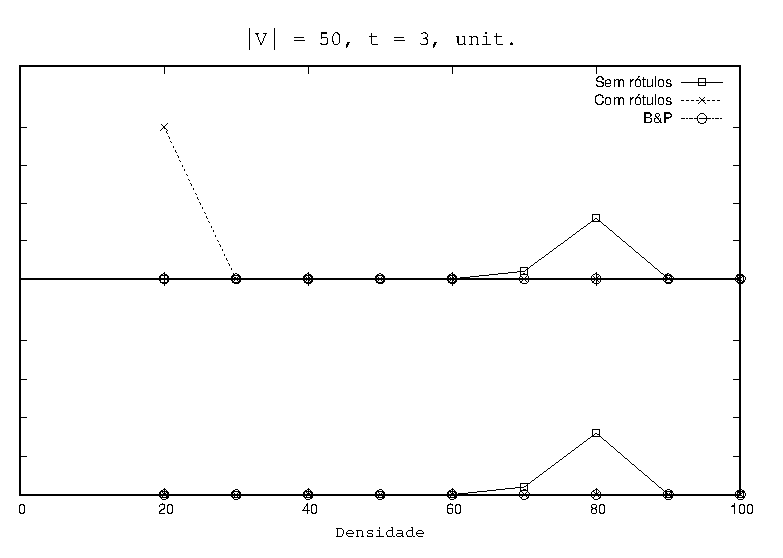
\includegraphics[scale=0.70]{figuras/2inst_den-sf3-s50-unit} }}%
    \caption{Quantidade de instâncias resolvidas para $t = 3$, peso unitário e ordem alta}%
    \label{fig:tree_sf3_s40_50_unit}%
\end{figure}

\begin{figure}[t]%
    \centering
    \subfloat{{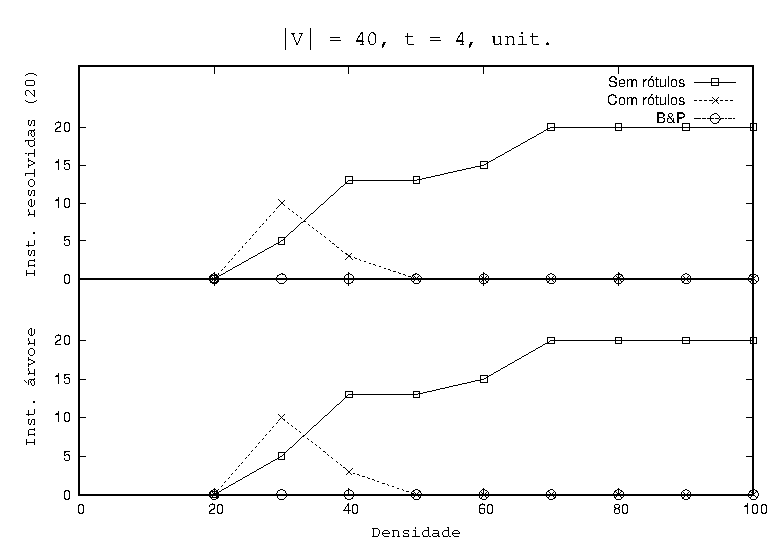
\includegraphics[scale=0.60]{figuras/2inst_den-sf4-s40-unit} }}%
    %\;
    \subfloat{{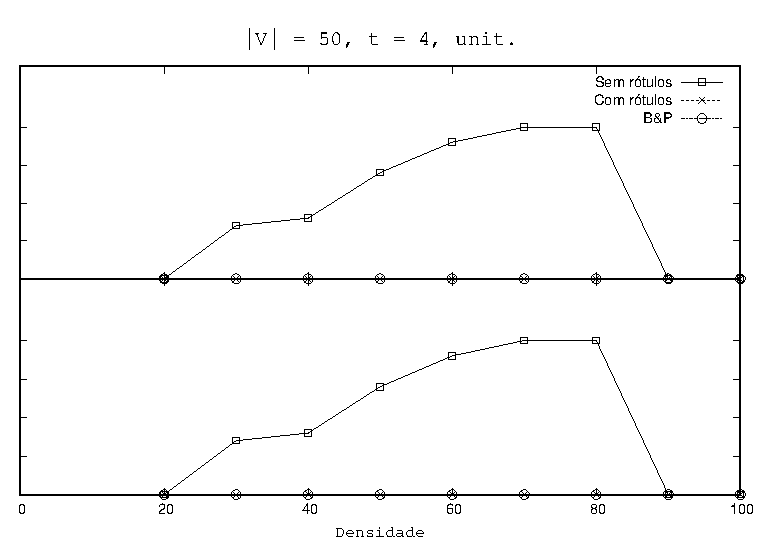
\includegraphics[scale=0.60]{figuras/2inst_den-sf4-s50-unit} }}    
    %% \subfloat[label 2]{{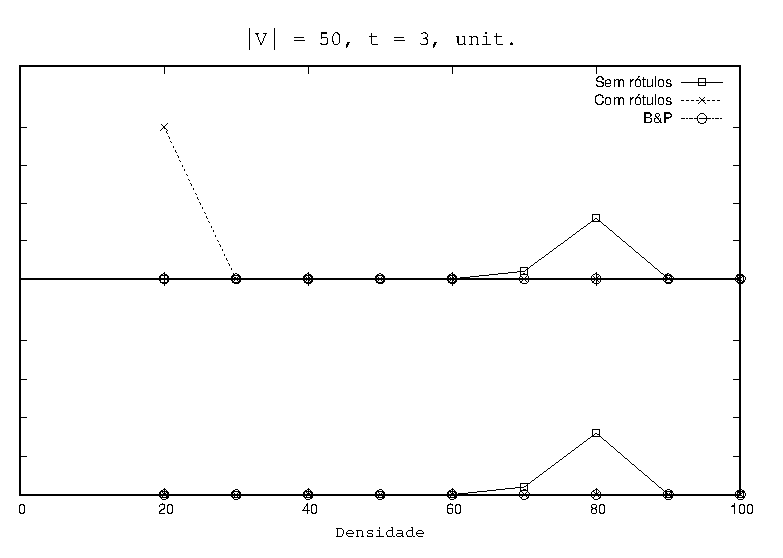
\includegraphics[scale=0.70]{figuras/2inst_den-sf3-s50-unit} }}%
    \caption{Quantidade de instâncias resolvidas para $t = 4$, peso unitário e ordem alta}%
    \label{fig:tree_sf4_s40_50_unit}%
\end{figure}

Nesta seção apresentamos os experimentos para o problema da árvore
$t$-spanner, comparando os desempenhos das formulações lineares
inteiras e da implementação do algoritmo de \emph{branch-and-price} que
descrevemos
para este problema. Ao longo deste capítulo, a formulação apresentada
na Seção~\ref{sec:form_mwstp} será denominada \emph{sem rótulos},
abreviada por \emph{SR}; e a formulação apresentada na
Seção~\ref{sec:form_mwstp_lab_dist} será denominada \emph{com
  rótulos}, abreviada por \emph{CR}. Por fim, a implementação do
algoritmo de \emph{branch-and-price} será chamada de \emph{B}\&\emph{P}.
Ao fim desta seção, apresentamos um quadro
resumo indicando em quais situações cada algoritmo exato é mais
indicado.

Ao longo deste capítulo, os gráficos que mostram somente informações
relativas à quantidade de instâncias resolvidas têm o seguinte
formato: a parte superior mostra a quantidade de instâncias
resolvidas, e a parte inferior mostra a quantidade de soluções ótimas,
que são árvores. A quantidade de instâncias totais, para as quais
foram realizados os experimentos, está dentro dos parênteses ao lado
do eixo das ordenadas.  Para todo gráfico mostrado neste capítulo, na
parte superior do gráfico são indicados os parâmetros que
foram fixados assim como seus respectivos valores.  Os grafos com
pesos aleatórios e com valores mais espaçados serão abreviados por
\emph{aleat}.  Já os grafos com pesos aleatórios mas com valores menos
espaçados serão abreviados por \emph{aleat. menor}. Abreviaremos os
grafos com pesos unitários por \emph{unit}.

Iniciamos os experimentos com grafos de ordem até 50.  As
Figuras~\ref{fig:tree_sf3_s40_50_unit}~e~\ref{fig:tree_sf4_s40_50_unit}
mostram a quantidade de instâncias resolvidas com pesos unitários
e ordens 40 e 50.  Pela Figura~\ref{fig:tree_sf3_s40_50_unit}, podemos
observar que, para os casos com pesos unitários e com densidades
maiores, a formulação~SR resolveu mais instâncias do que a
formulação~CR. Este comportamento fica mais claro quando o fator de
dilatação é maior, como ilustrado na
Figura~\ref{fig:tree_sf4_s40_50_unit}.  Para grafos pequenos (em
termos de densidade e ordem) com pesos unitários e com fator de
dilatação baixo (ou seja, menos opções a serem analisadas pelo
resolvedor), a formulação~CR teve um desempenho melhor do que a 
formulação~SR, como vemos na
Figura~\ref{fig:tree_sf3_s20_30_unit}. Este comportamento também é
visto para os valores de densidade baixa na
Figura~\ref{fig:tree_sf3_s40_50_unit}.

\begin{figure}%
    \centering
    \subfloat{{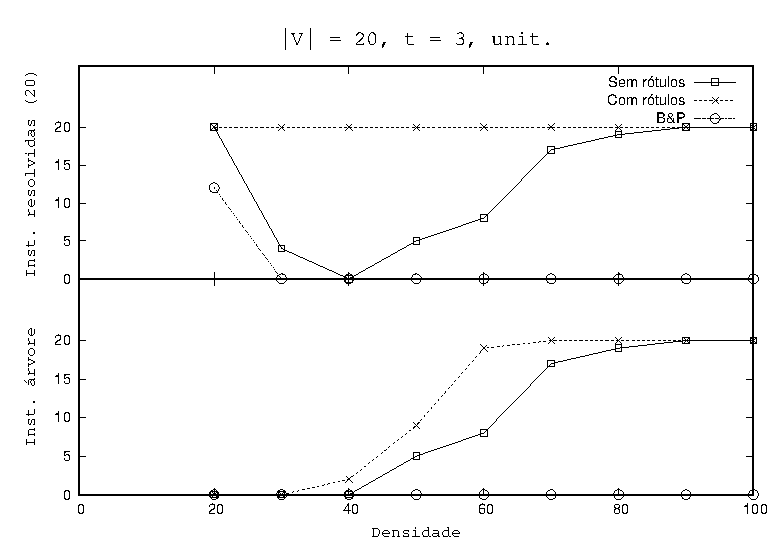
\includegraphics[scale=0.60]{figuras/2inst_den-sf3-s20-unit} }}%
    %\;
    \subfloat{{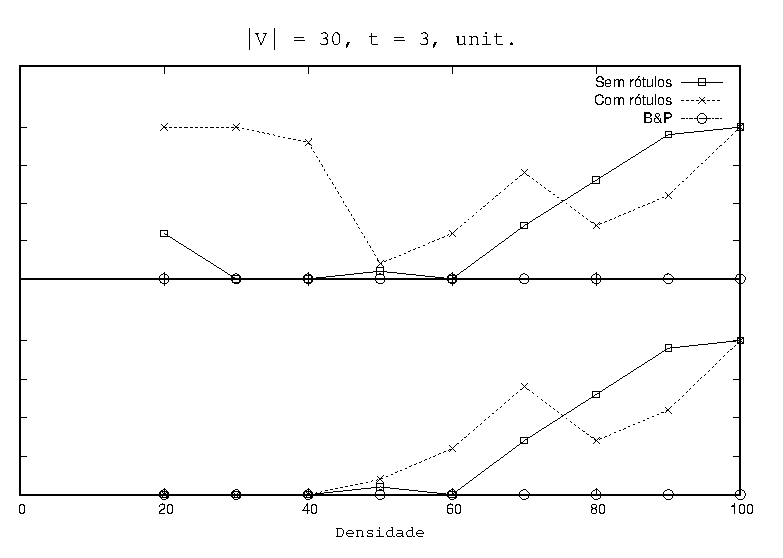
\includegraphics[scale=0.60]{figuras/2inst_den-sf3-s30-unit} }}    
    %% \subfloat[label 2]{{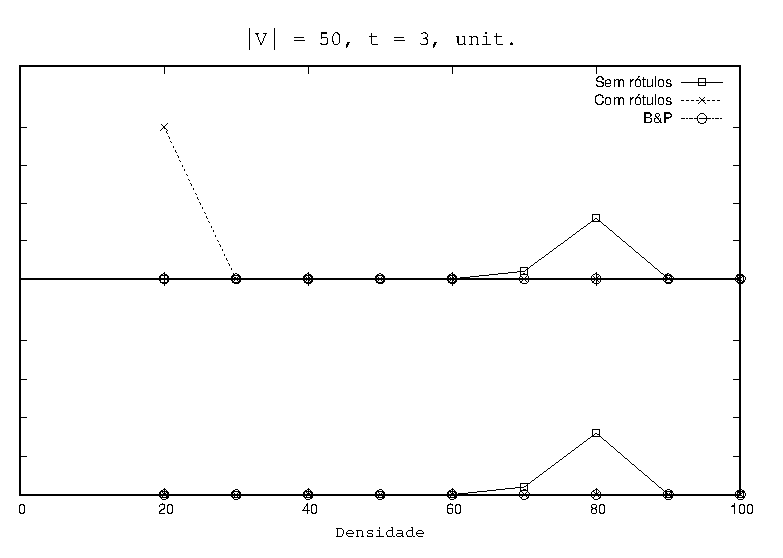
\includegraphics[scale=0.70]{figuras/2inst_den-sf3-s50-unit} }}%
    \caption{Quantidade de instâncias resolvidas para $t = 3$, peso unitário e ordem baixa}%
    \label{fig:tree_sf3_s20_30_unit}%
\end{figure}

Para instâncias com pesos aleatórios menos espaçados, a formulação~CR
mostrou-se melhor do que a formulação~SR em todas as situações,
considerando grafos com ordem até 50.  O fato interessante é que à
medida que a ordem do grafo ou o fator de dilatação aumenta, ambas as
formulações vão resolvendo menos instâncias até que, para ordem~50 e
fator de dilatação grande (quatro), B\&P tem desempenho
melhor (veja Figura~\ref{fig:2inst_den-sf4-s50-small_random}).  Já
para instâncias com pesos mais espaçados, o comportamento das
formulações SR e CR é semelhante, com a diferença de que a degradação
acontece de maneira um pouco mais acentuada (veja Figura~\ref{fig:tree_sf4_s20_50_random}).

\begin{figure}[t]
  \centering
  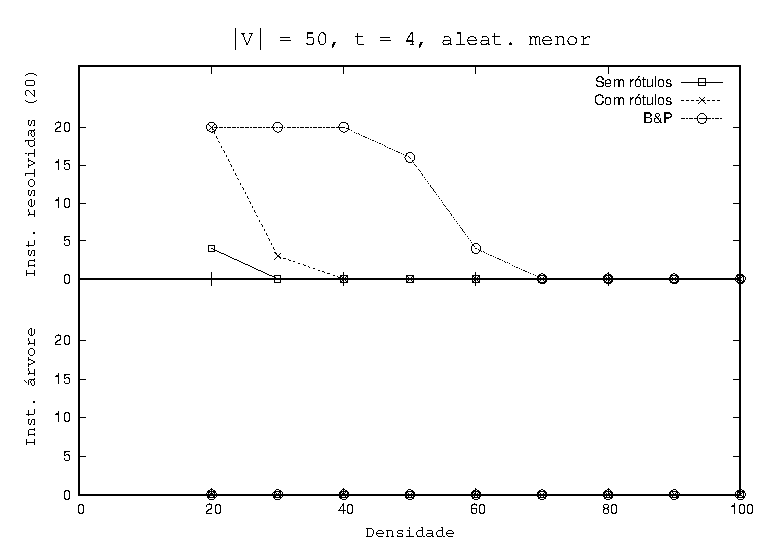
\includegraphics[scale=0.65]{figuras/2inst_den-sf4-s50-small_random} % era 0.35
  \caption{Quantidade de instâncias resolvidas para $t = 4$, peso aleatório menos espaçado e $|V| = 50$}
  \label{fig:2inst_den-sf4-s50-small_random}
\end{figure}

\begin{figure}%
    \centering
    \subfloat{{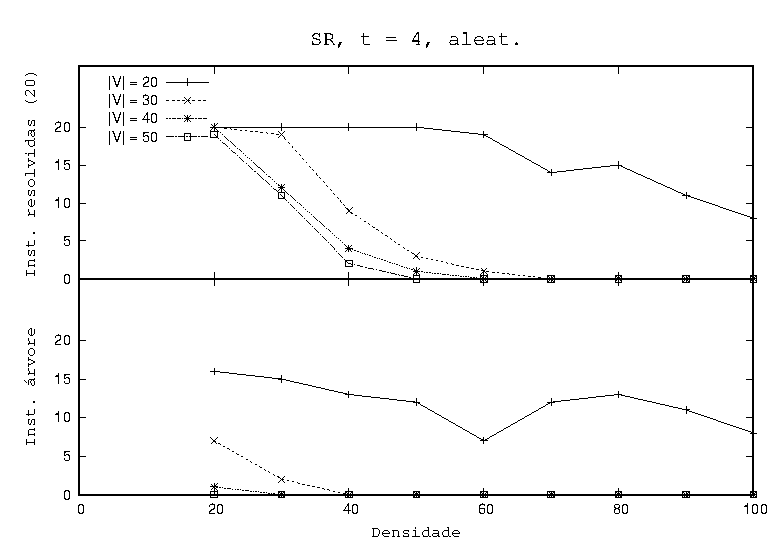
\includegraphics[scale=0.60]{figuras/find-2inst_den-sf4-s20_50-random} }}%
    %\;
    \subfloat{{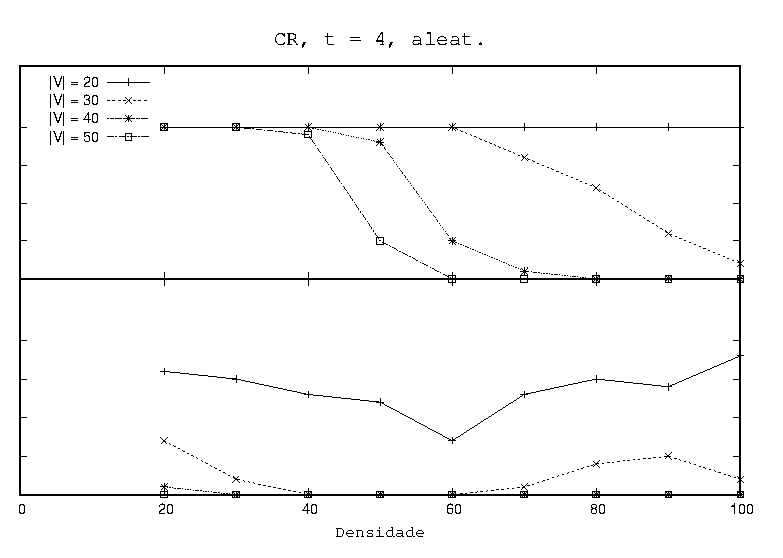
\includegraphics[scale=0.60]{figuras/labels-2inst_den-sf4-s20_50-random} }}
    \caption{Quantidade de instâncias resolvidas para $t = 4$ e peso aleatório}%
    \label{fig:tree_sf4_s20_50_random}%
\end{figure}


Notamos que, no caso de instâncias que admitem uma árvore $t$-spanner,
com pesos unitários, quando o fator de dilatação é alto (quatro), as
curvas dos desempenhos de uma mesma formulação nos gráficos superior e
inferior são as mesmas (veja
Figura~\ref{fig:tree_sf4_s40_50_unit}). Em outras palavras, para cada
instância resolvida, esta admite uma árvore $t$-spanner. Mesmo para o
fator de dilatação três, quando as densidades são mais altas, as curvas são as
mesmas (veja o lado direito das
Figuras~\ref{fig:tree_sf3_s40_50_unit}~e~\ref{fig:tree_sf3_s20_30_unit}).

Para instâncias com pesos aleatórios menos espaçados, o único caso em
que foram encontradas árvores $t$-spanner como solução são aquelas com
ordem~20 e com fator de dilatação quatro. No caso de pesos aleatórios mais
espaçados, o comportamento é semelhante.

Vamos analisar agora o desempenho das formulações SR e CR quando o
tempo limite de simulação é maior. Novamente consideramos a ordem
variando entre $20$ e $50$ e a densidade entre $20\%$ e $100\%$.  Para
instâncias com pesos aleatórios menos espaçados, ambas as formulações
SR e CR se comportam de maneira semelhante à situação onde o tempo de
simulação foi menor, descrita anteriormente. Além do desempenho de CR
ter sido melhor, para o fator de dilatação três e para grafos de ordens 20
e 30, todas as instâncias foram resolvidas utilizando esta formulação, exceto
para densidade de 20\%. Para os outros valores de ordem, a
Figura~\ref{fig:tree_sf3_s40_50_small_random_high_time} ilustra o
comportamento das duas formulações. Já para o fator quatro, quando as
ordens são altas, quase nenhuma instância foi resolvida. Para ordens
menores, veja a
Figura~\ref{fig:tree_sf4_s20_30_small_random_high_time}.  Para fatores
de dilatação três e quatro, e para os valores de ordem testados, quando a
densidade é mínima (20\%), a formulação~SR mostrou-se sempre melhor do
que a formulação~CR. Mais especificamente, com CR não foi possível
resolver nenhuma instância, enquanto que com SR foi possível revolver
a maioria das instâncias.

\begin{figure}%
    \centering
    \subfloat{{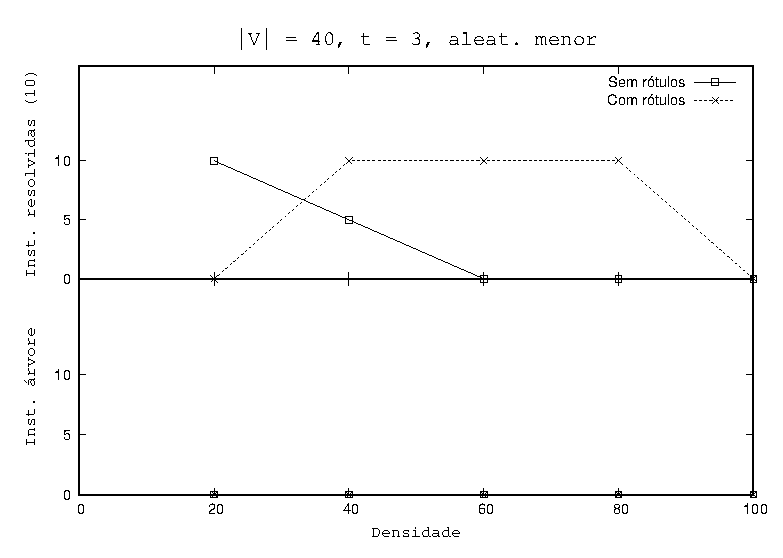
\includegraphics[scale=0.60]{figuras/2inst_den-sf3-s40-small_random-high_time} }}%
    %\;
    \subfloat{{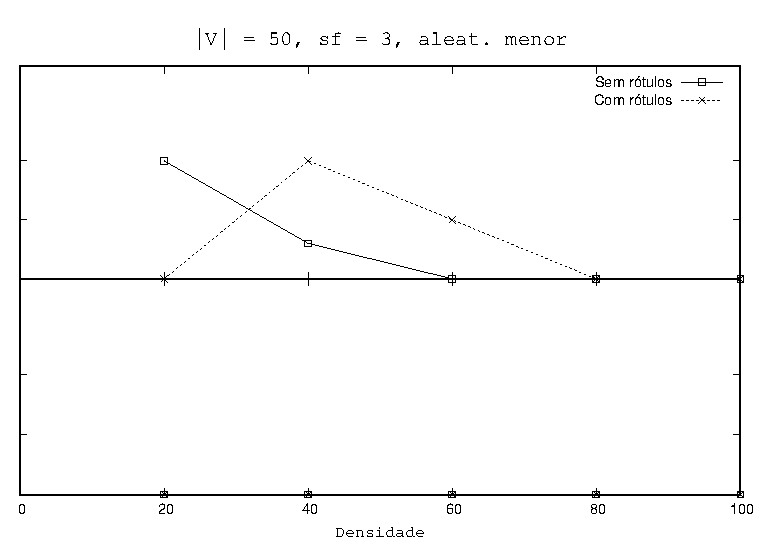
\includegraphics[scale=0.60]{figuras/2inst_den-sf3-s50-small_random-high_time} }}    
    %% \subfloat[label 2]{{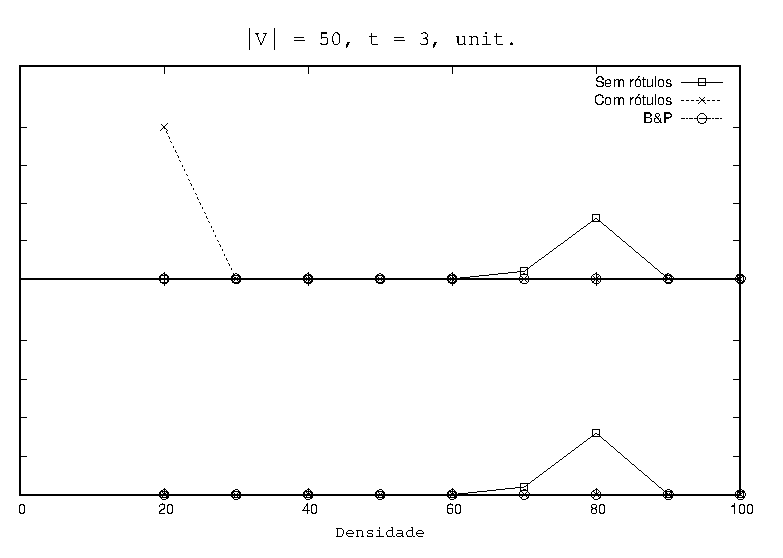
\includegraphics[scale=0.70]{figuras/2inst_den-sf3-s50-unit} }}%
    \caption{Quantidade de instâncias resolvidas para $t = 3$, peso
      aleatório menos espaçado, ordem alta e com tempo limite de
      3600 segundos}%
    \label{fig:tree_sf3_s40_50_small_random_high_time}%
\end{figure}

\begin{figure}%
    \centering
    \subfloat{{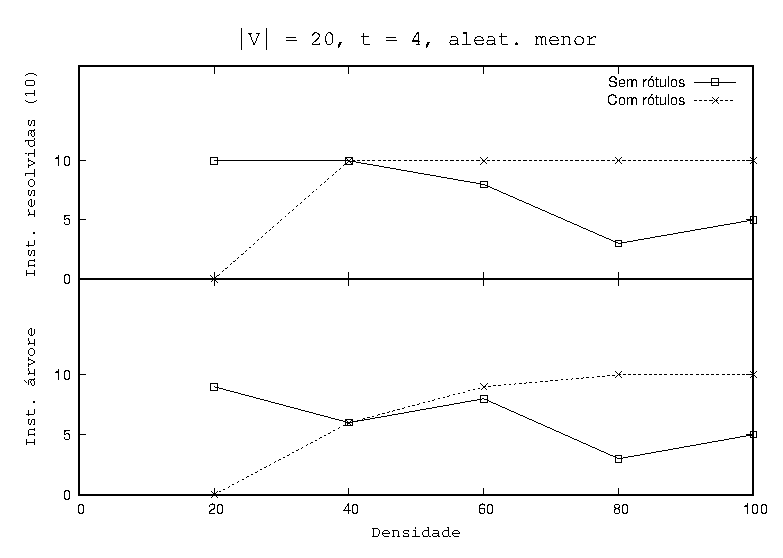
\includegraphics[scale=0.60]{figuras/2inst_den-sf4-s20-small_random-high_time} }}%
    %\;
    \subfloat{{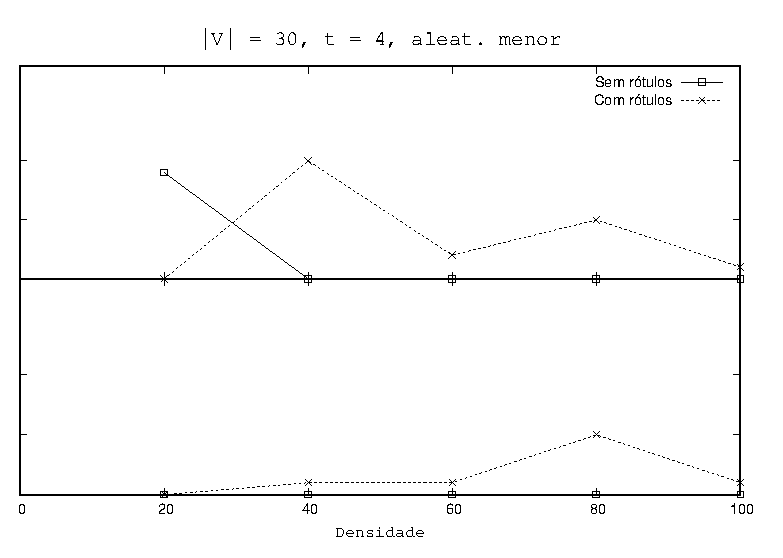
\includegraphics[scale=0.60]{figuras/2inst_den-sf4-s30-small_random-high_time} }}    
    %% \subfloat[label 2]{{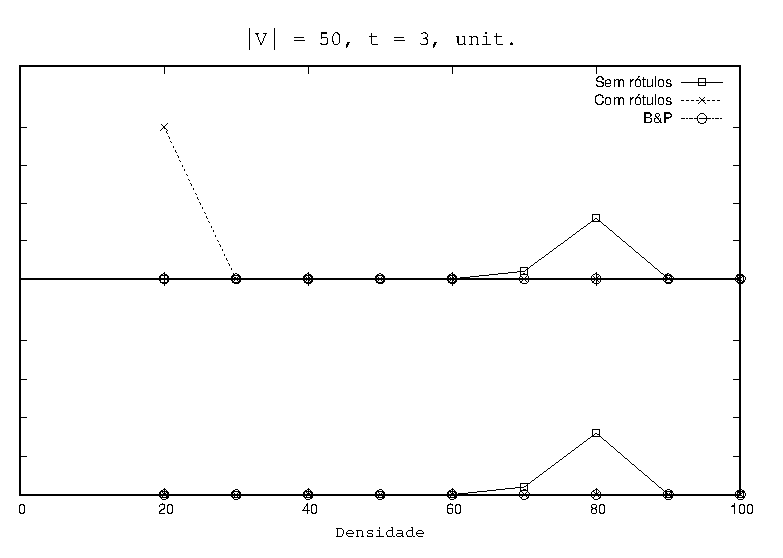
\includegraphics[scale=0.70]{figuras/2inst_den-sf3-s50-unit} }}%
    \caption{Quantidade de instâncias resolvidas para $t = 4$, peso
      aleatório menos espaçado, ordem baixa e com tempo limite de 3600
      segundos}%
    \label{fig:tree_sf4_s20_30_small_random_high_time}%
\end{figure}


Realizamos experimentos com grafos de ordem maior: entre 60 e 80.
Para o caso de pesos aleatórios menos espaçados, consideramos
densidades de até 50\%.  Para pesos unitários, variamos a densidade
entre 20\% e 80\%.  Consideramos valores de densidade maiores para
pesos unitários, em decorrência do comportamento das curvas nas
densidades maiores apresentadas nas
Figuras~\ref{fig:tree_sf3_s40_50_unit}~e~\ref{fig:tree_sf4_s40_50_unit}.
Para cada combinação, testamos 10~instâncias. Como mencionado no
início do capítulo, o limite de tempo para este cenário foi de 3600
segundos.

Considerando pesos aleatórios menos espaçados, à medida que a ordem
e/ou densidade e/ou fator de dilatação cresce, o número de instâncias
resolvidas por CR
decresce, como vemos na
Tabela~\ref{tab:tree_labels_small_random_big_size}.  Para o fator de
dilatação quatro, ocultamos as linhas para as combinações para as quais
não foi possível resolver nenhuma instância. Para a formulação~SR, o
comportamento é semelhante ao descrito acima, ilustrado na
Tabela~\ref{tab:tree_find_small_random_big_size}. Esta tabela não
mostra dados para o fator de dilatação quatro pois nenhuma instância foi
resolvida.  Observamos que o comportamento do resolvedor (CPLEX)
utilizando ambas as formulações
para ordem e limite de tempo maiores é semelhante ao caso em que a
ordem e o limite de tempo são menores, como abordado anteriormente.

\begin{center}
\noindent
\footnotesize{
\begin{tabular}{|c|c|c|c|c|}\hline
{$t$} & {Densidade (\%)} & {Ordem} & {\# Inst. resolvidas} & {Tempo (s)}
\\ \hline\hline
%\multirow{12}{*}{3} & 10 & 20 & 0 & 0 & 10 & 0.01  \\
%\multirow{11}{*}{3} & 10 & 40 & 5 & 0 & 5  & 0.02 \\
\multirow{12}{*}{3}	&	20	&	60	&	10	&	$\num{1,3603393}$	\\
	&	30	&	60	&	10	&	$\num{6,246502}$	\\
	&	40	&	60	&	9	&	$\num{13,8250511111111}$	\\
	&	50	&	60	&	0	&	0	\\
	&	20	&	70	&	10	&	$\num{3,462295}$	\\
	&	30	&	70	&	10	&	$\num{11,25421}$	\\
	&	40	&	70	&	0	&	0	\\
	&	50	&	70	&	0	&	0	\\
	&	20	&	80	&	10	&	$\num{7,913799}$	\\
	&	30	&	80	&	5	&	$\num{23,89124}$	\\
	&	40	&	80	&	0	&	0	\\
&	50	&	80	&	0	&	0	\\
\hline
\multirow{3}{*}{4}	&	20	&	60	&	9	&	$\num{20,5626644444444}$	\\
	%% &	30	&	60	&	0	&	0	\\
	%% &	40	&	60	&	0	&	0	\\
	%% &	50	&	60	&	0	&	0	\\
	&	20	&	70	&	7	&	$\num{66,0951857142857}$	\\
	%% &	30	&	70	&	0	&	0	\\
	%% &	40	&	70	&	0	&	0	\\
	%% &	50	&	70	&	0	&	0	\\
	&	20	&	80	&	4	&	$\num{168,88825}$	\\
	%% &	30	&	80	&	0	&	0	\\
	%% &	40	&	80	&	0	&	0	\\
	%% &	50	&	80	&	0	&	0	\\
\hline\hline
\end{tabular}
}
\captionof{table}{Quantidade de instâncias resolvidas com a formulação CR para peso aleatório menos espaçado}\label{tab:tree_labels_small_random_big_size}
\end{center}


\begin{center}
\noindent
\footnotesize{
\begin{tabular}{|c|c|c|c|c|}\hline
{$t$} & {Densidade (\%)} & {Ordem} & {\# Inst. resolvidas} & {Tempo (s)}
\\ \hline\hline
\multirow{12}{*}{3}	&	20	&	60	&	10	&	$\num{8,591142}$	\\
	&	30	&	60	&	6	&	$\num{189,917166666667}$	\\
	&	40	&	60	&	1	&	$\num{303,133}$	\\
	&	50	&	60	&	0	&	$\num{0}$	\\
	&	20	&	70	&	10	&	$\num{86,58809}$	\\
	&	30	&	70	&	4	&	$\num{529,29025}$	\\
	&	40	&	70	&	0	&	$\num{0}$	\\
	&	50	&	70	&	0	&	$\num{0}$	\\
	&	20	&	80	&	10	&	$\num{159,62539}$	\\
	&	30	&	80	&	1	&	$\num{610,231}$	\\
	&	40	&	80	&	0	&	$\num{0}$	\\
	&	50	&	80	&	0	&	$\num{0}$	\\
\hline\hline
\end{tabular}
}
\captionof{table}{Quantidade de instâncias resolvidas com a formulação SR para peso aleatório menos espaçado}\label{tab:tree_find_small_random_big_size}
\end{center}

Para o caso unitário, enquanto CR só conseguiu resolver algumas
instâncias para o fator de dilatação três, SR só conseguiu resolver
algumas instâncias para o fator de dilatação quatro (veja Tabelas~\ref{tab:tree_labels_unit_big_size}~e~\ref{tab:tree_find_unit_big_size})
Em ambos os casos, só
instâncias com densidades mínimas (20\%) puderam ser resolvidas.
%% Assim como para o caso aleatório menos espaçado, aqui o comportamento dos
%% algoritmos se assemelha ao caso em que a ordem e o tempo de
%% simulação são menores, como mostrado nas
%% Figuras~\ref{fig:tree_sf3_s40_50_unit}~e~\ref{fig:tree_sf4_s40_50_unit}.


\begin{center}
\noindent
\footnotesize{
\begin{tabular}{|c|c|c|c|c|}\hline
{$t$} & {Densidade (\%)} & {Ordem} & {\# Inst. resolvidas} & {Tempo (s)}
\\ \hline\hline
\multirow{3}{*}{3}	&	20	&	60	&	5	&	$\num{14,457256}$	\\
	%% &	30	&	60	&	0	&	$\num{0}$	\\
	%% &	40	&	60	&	0	&	$\num{0}$	\\
	%% &	50	&	60	&	0	&	$\num{0}$	\\
	&	20	&	70	&	1	&	$\num{32,0276}$	\\
	%% &	30	&	70	&	0	&	$\num{0}$	\\
	%% &	40	&	70	&	0	&	$\num{0}$	\\
	%% &	50	&	70	&	0	&	$\num{0}$	\\
	&	20	&	80	&	1	&	$\num{36,5025}$	\\
	%% &	30	&	80	&	0	&	$\num{0}$	\\
	%% &	40	&	80	&	0	&	$\num{0}$	\\
	%% &	50	&	80	&	0	&	$\num{0}$	\\
\hline\hline
\end{tabular}
}
\captionof{table}{Quantidade de instâncias resolvidas com a formulação CR para peso unitário}\label{tab:tree_labels_unit_big_size}
\end{center}

\begin{center}
\noindent
\footnotesize{
\begin{tabular}{|c|c|c|c|c|}\hline
{$t$} & {Densidade (\%)} & {Ordem} & {\# Inst. resolvidas} & {Tempo (s)}
\\ \hline\hline
\multirow{2}{*}{4}	&	20	&	60	&	5	&	$\num{185,242}$
	\\
	&	20	&	70	&	1	&	$\num{617,6485}$
\\
\hline\hline
\end{tabular}
}
\captionof{table}{Quantidade de instâncias resolvidas com a formulação SR para peso unitário}\label{tab:tree_find_unit_big_size}
\end{center}


Analisamos também os casos em que os fatores de dilatação são baixos.
\sisetup{round-mode=places,round-precision=1}
Mais especificadamente, executamos simulações para os valores $\num{1,1}$
\sisetup{round-mode=places,round-precision=0}
e~$2$. Para ambos os valores, só consideramos os casos em que os pesos
são aleatórios (tanto os menos espaçados como os mais espaçados).
Lembre-se que, para o fator de dilatação dois, o problema é fácil para
o caso unitário (veja Tabela~\ref{tab:t-spanner_opt}). Variamos as
densidades entre $20\%$ e $100\%$. Variamos as ordens entre 20 e 50.
Para cada combinação, consideramos 20 instâncias (e tempo limite de
execução de 1800 segundos).

Com a formulação CR todas as instâncias foram resolvidas em menos de
três segundos. Apesar disso, nenhuma das instâncias consideradas admite
uma árvore $t$-spanner como solução. A formulação~SR teve pior
desempenho também neste cenário.  Pela
Figura~\ref{fig:tree_sf1_1_sf2_s50_aleat}, percebemos que o tempo de
execução foi bem diferente do que obtivemos com a formulação~CR.  Além
disso, notamos que SR não escala bem com o aumento da densidade e/ou
com o aumento da ordem. Ademais, para a combinação de ordem~50 com
densidade pelo menos~80 e com pesos aleatórios menos espaçados,
algumas das instâncias não foram resolvidas, piorando a situação com o
aumento da densidade. Isto nos dá um indicativo de que, para este tempo
limite de execução, para ordens maiores do que 50 e densidades altas,
provavelmente já não seria possível resolver tais instâncias.

\begin{figure}%
    \centering
    \subfloat{{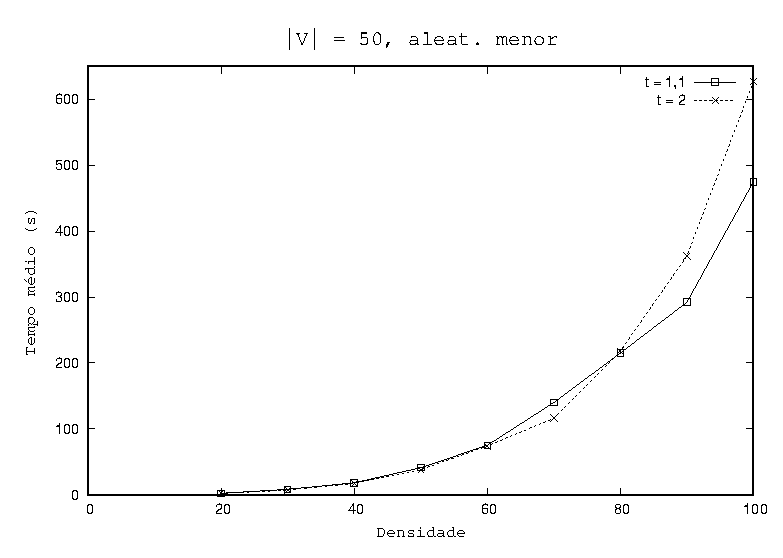
\includegraphics[scale=0.60]{figuras/time_den-sf1_1-sf2-s50-small_random} }}%
    %\;
    \subfloat{{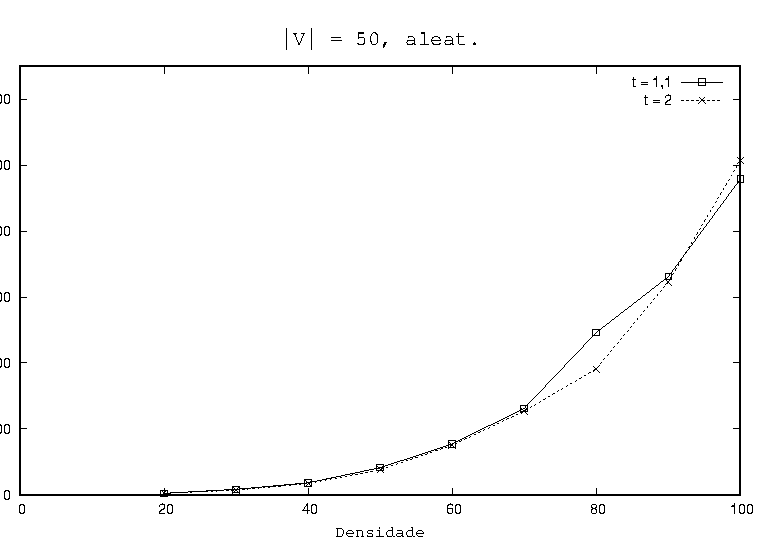
\includegraphics[scale=0.60]{figuras/time_den-sf1_1-sf2-s50-random} }}    
    %% \subfloat[label 2]{{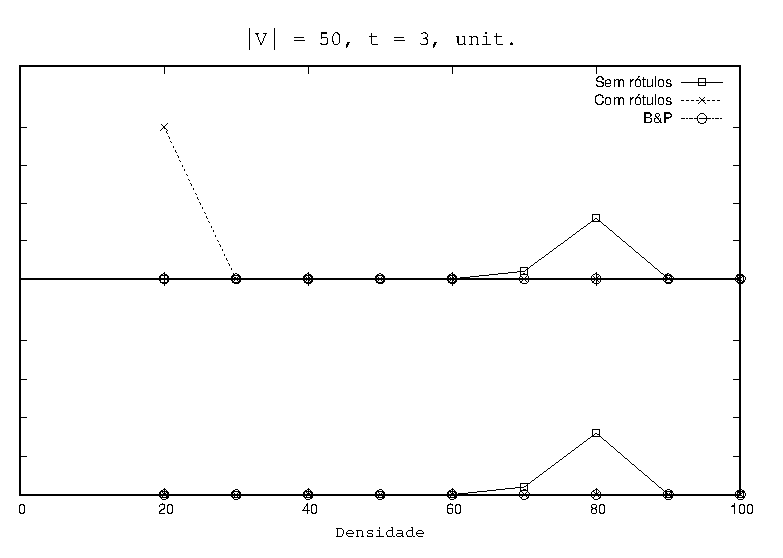
\includegraphics[scale=0.70]{figuras/2inst_den-sf3-s50-unit} }}%
    \caption{Tempo médio para instâncias resolvidas com a formulação SR para $|V| = 50$ e $t$ baixo}%
    \label{fig:tree_sf1_1_sf2_s50_aleat}%
\end{figure}

Tendo por base os experimentos que realizamos em diversos cenários,
apresentamos na Tabela~\ref{tab:conc_alg_exato} a nossa recomendação
quanto ao uso de cada formulação, dependendo dos tipos das
instâncias. Representamos os valores (representados por adjetivos) dos
parâmetros por meio dos seguintes grupos:
\begin{itemize}
\item Ordem (Ord.): \emph{pequena} para valores até 40; \emph{grande} para
  valores maiores do que 40;
\item Densidade (Dens.): \emph{baixa} para valores até 40\%; \emph{alta}
  para valores maiores do que 40\%;
\item Fator de dilatação ($t$): \emph{baixo} para valores até três; \emph{alto} para
  o valor quatro;
\item Peso (P.): \emph{unitário} (unit.); \emph{aleatório} (aleat.) para
  pesos aleatórios menos espaçados e mais espaçados.
\end{itemize}

Na Tabela~\ref{tab:conc_alg_exato}, para cada combinação de valores de
parâmetros, é indicada a formulação que achamos mais adequada. Quando
duas formulações são mostradas, a segunda (dentro de parênteses) é utilizada em
situações específicas. Quando o sinal de igual (=) é mostrado,
significa que o desempenho das duas formulações são semelhantes.

\begin{table}
\centering

\begin{tabular}{llcccccc}
\toprule
%\textbf{Dens} & \textbf{Ordem} & \multicolumn{4}{c}{\textbf{Fator de dilatação}} \\
%\cmidrule{3-6}
& & \multicolumn{2}{c}{$t$ baixo} & \multicolumn{2}{c}{$t$ alto}\\
\cmidrule[0.05ex]{3-6}
%& & \multicolumn{4}{c}{\textbf{Peso}} \\
%% \cmidrule{3-6}
& & P. unit. & P. aleat. & P. unit. & P. aleat. \\
\midrule[0.1ex]
Dens. alta & Ord. grande & SR & CR & SR & = \\ 
    &  Ord. peq. & SR (CR) & CR & CR & CR \\
\addlinespace
Dens. baixa & Ord. grande & CR & CR & SR & CR (SR) \\ 
    & Ord. peq. & CR & CR & CR (SR) & CR \\ 
\bottomrule
\end{tabular}
\caption{Recomendação de uso das formulações SR e CR}\label{tab:conc_alg_exato}
\end{table}

Pelos experimentos, observamos que quanto maior a variação no peso das
arestas, maior a vantagem em utilizar CR (podemos observar isso nas
colunas da Tabela~\ref{tab:conc_alg_exato} relativas a pesos
aleatórios). O domínio de CR fica claro quando se considera pesos
aleatórios mais espaçados (apenas no caso de pesos aleatórios menos
espaçados, $t$ alto, densidade de 20\% e ordem de 50, a formulação~SR
mostrou-se melhor).

Para pesos unitários e com densidade alta, em geral, SR é melhor
(exceto para o caso de ordem pequena). Neste caso, apenas para $t$ baixo ($t = 3$),
densidade alta e ordem 20, a formulação~CR mostrou-se melhor.

O último caso específico ilustrado na Tabela~\ref{tab:conc_alg_exato}
é para pesos unitários, com densidade baixa, $t$~alto e
ordem~40. Neste cenário, SR mostrou-se melhor do que CR.

Outro fato exibido na Tabela~\ref{tab:conc_alg_exato} é que, para
densidades baixas, quase sempre a formulação CR é melhor. O único caso
(dos oito possíveis) em que SR foi melhor foi para $t$ alto, pesos
unitários, densidade baixa e ordem grande.


\section{Resultados para  $t$-spanner de peso mínimo}

Nesta seção apresentamos os resultados dos experimentos
para testar a implementação do algoritmo de \emph{branch-and-price}
para o problema de $t$-spanner de peso mínimo, representada pela
sigla~\emph{B}\&\emph{P}. Nós não apresentaremos experimentos para a
formulação apresentada no Capítulo~\ref{cap:mwsp} pois 
alguns experimentos iniciais mostraram que a
formulação não apresentava um bom desempenho.
Com relação à implementação do algoritmo de \emph{branch-and-price}, 
utilizamos como base os mesmos experimentos
realizados por Sigurd e Zachariasen~\cite{SigurdZ2004}. Além dos
valores de parâmetros utilizados pelos autores (que são subconjuntos
dos valores apresentados na Seção~\ref{sec:parametros}), adicionamos
novos valores de parâmetros. Mais especificamente, para a ordem dos
grafos, em alguns casos, além dos valores do conjunto
$\{16, 32, 64\}$, também testamos os valores $80$, $90$ e
$100$. Para o fator de dilatação, além dos valores do conjunto
\sisetup{round-mode=places,round-precision=1}
$\{\num{1,1}; 2; 4\}$, também incluímos o valor três. Além destes novos
\sisetup{round-mode=places,round-precision=0}
valores de parâmetros, também variamos a densidade do grafo, entre
valores de 20\% e 80\%.  Por fim, consideramos experimentos com mais
tempo limite de execução, passando a ter como limite o valor de
3600~segundos. Como mencionado na Seção~\ref{sec:parametros}, para cada
combinação de parâmetros foram criadas 10 instâncias.  Ao longo desta
seção, quando nos referirmos aos pesos aleatórios, estaremos nos
referindo apenas à classe dos mais espaçados.


\begin{table}
  \centering
\scalebox{0.7}{
\begin{tabular}{|l|rrrrrr|rrrrrr|}
  %\toprule
  \hline
%Peso & \multicolumn{12}{c|}{Aleatório} \\
%\cmidrule[0.05ex]{2-25}
Grau & \multicolumn{6}{c|}{$4$} & \multicolumn{6}{c|}{$8$} \\
%\cmidrule[0.05ex]{2-25}
Ordem & 16 & 32 & 64 & 80 & 90 & 100 & 16 & 32 & 64 & 80 & 90 & 100 \\
%\midrule[0.1ex]
\hline
\hline
\sisetup{round-mode=places,round-precision=1}
$t = \num{1,1}$ & $(10)$ & $(10)$ & $(10)$ & - & - & - & $(10)$ & $(10)$ & $(10)$ & - & - & -
\sisetup{round-mode=places,round-precision=0}
%& 0 & 0 & 0 & 0 & 0 & 0 & 0 & 0 & 0 & 0 & 0 & 0
\\ 
%\addlinespace
$t = 2$ & $(10)$ & $(10)$ & $(10)$ & - & - & - & $(10)$ & $(10)$ & $\num{6,408482} (10)$ & - & - & -
%& 0 & 0 & 0 & 0 & 0 & 0 & 0 & 0 & 0 & 0 & 0 & 0
\\ 
%\bottomrule
$t = 3$ & $(10)$ & $(10)$ & $\num{10,1925287} (10)$ & $\num{7,824523} (10)$ & $\num{7,7401784} (10)$ & $\num{202,475267} (10)$ & $(10)$ & $\num{289,664214} (10)$ & $\num{133,767214285714} \;\,(7)$ & $\num{591,4651} \;\,(8)$ & $\num{371,9923} \;\,(6)$ & $\num{1146,8458} \;\,(5)$
\\
$t = 4$ & $(10)$ & $(10)$ & $\num{99,7693944444444} (10)$ & - & - & - & $\num{22,662389} (10)$ & $\num{709,6701} \;\,(6)$ & $\num{1157} \;\,(1)$ & - & - & -
\\
\hline
\end{tabular}
}
\caption{Quantidade de instâncias resolvidas por B\&P e tempo médio de execução para peso aleatório}\label{tab:mwsp_random}
\end{table}


\begin{table}
  \centering
\scalebox{0.7}{
\begin{tabular}{|l|rrrrrr|rrrrrr|}
  %\toprule
  \hline
%Peso & \multicolumn{12}{c|}{Dist. euclid.} \\
%\cmidrule[0.05ex]{2-25}
Grau & \multicolumn{6}{c|}{$4$} & \multicolumn{6}{c|}{$8$} \\
%\cmidrule[0.05ex]{2-25}
Ordem & 16 & 32 & 64 & 80 & 90 & 100 & 16 & 32 & 64 & 80 & 90 & 100 \\
%\midrule[0.1ex]
\hline
\hline
\sisetup{round-mode=places,round-precision=1}
$t = \num{1,1}$ & $(10)$ & $(10)$ & $(10)$ & - & - & - & $(10)$ & $(10)$ & $(10)$ & - & - & -
\sisetup{round-mode=places,round-precision=0}
%& 0 & 0 & 0 & 0 & 0 & 0 & 0 & 0 & 0 & 0 & 0 & 0
\\ 
%\addlinespace
$t = 2$ & $(10)$ & $(10)$ & $(10)$ & - & - & - & $(10)$ & $(10)$ & $\num{5,387807} (10)$ & - & - & -
%& 0 & 0 & 0 & 0 & 0 & 0 & 0 & 0 & 0 & 0 & 0 & 0
\\
$t = 3$ & $(10)$ & $(10)$ & $(10)$ & $\num{5,2910455} (10)$ & $(10)$ & $\num{7,7604249} (10)$ & $(10)$ & $\num{49,224839} (10)$ & $\num{675,009777777778} \;\,(9)$ & $\num{744,797222222222} \;\,(9)$ & $\num{596,4886} (10)$ & $\num{667,042375} \;\,(8)$
\\
$t = 4$ & $(10)$ & $\num{6,1226376} (10)$ & $\num{312,173572} (10)$ & - & - & - & $\num{163,913996} (10)$ & $\num{1708,26471428571} \;\,(7)$ & $0$ & - & - & -
\\
%\bottomrule
\hline
\end{tabular}
}
\caption{Instâncias resolvidas por B\&P e tempo médio de execução para distância euclidiana}\label{tab:mwsp_euclidean}
\end{table}


Inicialmente apresentamos os resultados computacionais obtidos
com o B\&P, para instâncias cujo parâmetro variado foi o
grau médio. Posteriormente mencionamos os resultados para instâncias de
densidades variadas.

As Tabelas~\ref{tab:mwsp_random}~e~\ref{tab:mwsp_euclidean}~e~\ref{tab:mwsp_unit}
mostram a quantidade de instâncias resolvidas (de um total de 10),
juntamente com o tempo médio de execução das instâncias
resolvidas. A quantidade de instâncias resolvidas está dentro de
parênteses, enquanto o tempo médio é mostrado ao lado esquerdo.  Tempos médios 
menores do que 5 segundos não são mostrados nas tabelas.  Quando
nenhuma instância é resolvida, é mostrado o valor zero. Para as
combinações em que não houve experimentos, aparece um traço~($-$).

Pelas Tabelas~\ref{tab:mwsp_random}~e~\ref{tab:mwsp_euclidean} podemos
observar que as instâncias são resolvidas rapidamente quando o fator de
\sisetup{round-mode=places,round-precision=1}
dilatação é $\num{1,1}$.  Ainda considerando tanto pesos aleatórios
\sisetup{round-mode=places,round-precision=0}
como distâncias
euclidianas, e fator de dilatação dois, todas as instâncias são
resolvidas rapidamente, mas já há uma diferença considerável para
instâncias de grau médio~8 e ordem~$64$.  Acreditamos que, a partir desta ordem
(e para grau médio oito), o
tempo de execução aumentará drasticamente e o número de instâncias
resolvidas cairá. A partir do fator três, os resultados começam a
diferir para os dois tipos de peso. Para pesos aleatórios, a partir da
ordem~$100$, os tempos aumentam consideravelmente.  Além disso, para
grau médio oito, é perceptível a queda no número de instâncias resolvidas à
medida que aumenta a ordem. Já para as distâncias euclidianas, a implementação
escala bem para grau médio quatro; e para grau médio oito, apesar do aumento no
tempo, percebemos que ainda podemos resolver instâncias de ordens
maiores. Considerando o fator de dilatação $t = 4$, 
percebemos que a implementação do B\&P se comporta melhor quando os pesos são
aletórios.  Para grau médio oito, para ambos os tipos de peso,
percebemos que a ordem~64 é o limite para
o tempo de execução que consideramos. 

\begin{table}
\centering
\begin{tabular}{|l|rrr|rrr|}\hline
%\toprule
%Peso & \multicolumn{6}{c|}{Unit.} \\
%\cmidrule[0.05ex]{2-7}
Grau & \multicolumn{3}{c|}{$4$} & \multicolumn{3}{c|}{$8$} \\
%\cmidrule[0.05ex]{2-7}
Ordem & 16 & 32 & 64 & 16 & 32 & 64 \\
%\midrule[0.1ex]
\hline
\hline
%$t = 1,1$ & $0$ & $0$ & $0$ & $(10)$ & $(10)$ & $(10)$ \\
%\addlinespace
$t = 2$ & $(10)$ & $\num{44,9659241} \;\,(9)$ & $\num{358,513257} \;(7)$ & $\num{1794,0113333} \;\,(3)$ & $0$ & $0$ \\
$t = 3$ & $\num{91,676334} \;\,(10)$ & $\num{674,031175}\;\,(4)$ & $0$ & $0$ & $0$ & $0$ \\
$t = 4$ & $\num{9,507818}\;\,(10)$ & $0$ & $0$ & $\num{1265,6445} \;\,(10)$ & $0$ & $0$ \\
%\bottomrule
\hline
\end{tabular}
\caption{Quantidade de instâncias resolvidas e tempo de execução para peso unitário}\label{tab:mwsp_unit}
\end{table}


Para o caso de pesos unitários, os resultados são semelhantes aos apresentados
nos experimentos realizados por Sigurd e Zachariasen
(veja Tabela~\ref{tab:mwsp_unit}). Para o fator de dilatação dois, tanto para
o grau quatro (e ordem $64$) como para grau oito (e ordem $16$), foi possível
resolver instâncias, diferentemente do que ocorreu nos experimentos de
Sigurd e Zachariasen.
%% Só nos foi possível resolver um conjunto maior de instâncias para grau médio
%% oito e fator de dilatação quatro.


%% \begin{table}
%%   \centering
%% \scalebox{0.7}{
%% \begin{tabular}{l|cccccccccccc|cccccccccccc|}
%%   %\toprule
%%   \hline
%% Peso & \multicolumn{12}{c|}{Dist. euclid.} & \multicolumn{12}{c|}{Aleat.}\\
%% %\cmidrule[0.05ex]{2-25}
%% Grau & \multicolumn{6}{c|}{$4$} & \multicolumn{6}{c|}{$8$} & \multicolumn{6}{c|}{$4$} & \multicolumn{6}{c|}{$8$} \\
%% %\cmidrule[0.05ex]{2-25}
%% Ordem & 16 & 32 & 64 & 80 & 90 & 100 & 16 & 32 & 64 & 80 & 90 & 100 & 16 & 32 & 64 & 80 & 90 & 100 & 16 & 32 & 64 & 80 & 90 & 100 \\
%% %\midrule[0.1ex]
%% $t = 1,1$ & 0 & 0 & 0 & 0 & 0 & 0 & 0 & 0 & 0 & 0 & 0 & 0 & 0 & 0 & 0 & 0 & 0 & 0 & 0 & 0 & 0 & 0 & 0 & 0 \\ 
%% %\addlinespace
%% $t = 2$ & 0 & 0 & 0 & 0 & 0 & 0 & 0 & 0 & 0 & 0 & 0 & 0 & 0 & 0 & 0 & 0 & 0 & 0 & 0 & 0 & 0 & 0 & 0 & 0 \\ 
%% %\bottomrule
%% \end{tabular}
%% }
%% \caption{Teste}\label{tab:mwsp}
%% \end{table}



\begin{figure}[t]%
    \centering
    \subfloat{{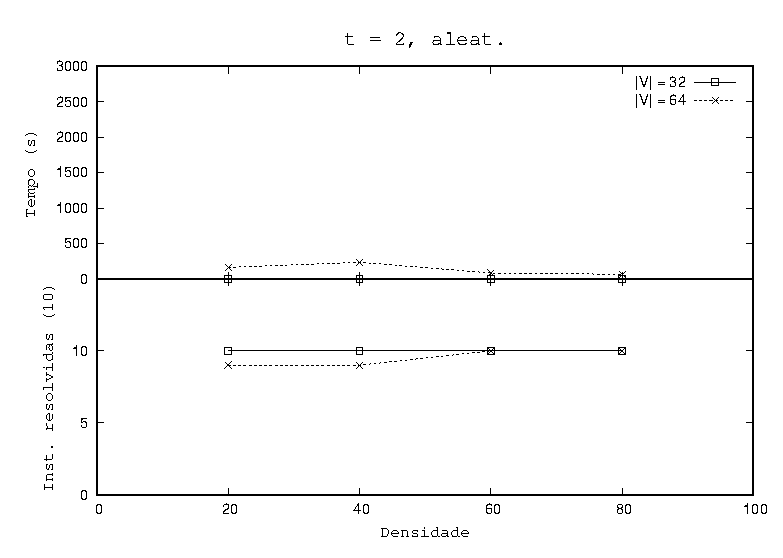
\includegraphics[scale=0.60]{figuras/time_inst_den-sf2-random} }}%
    %\;
    \subfloat{{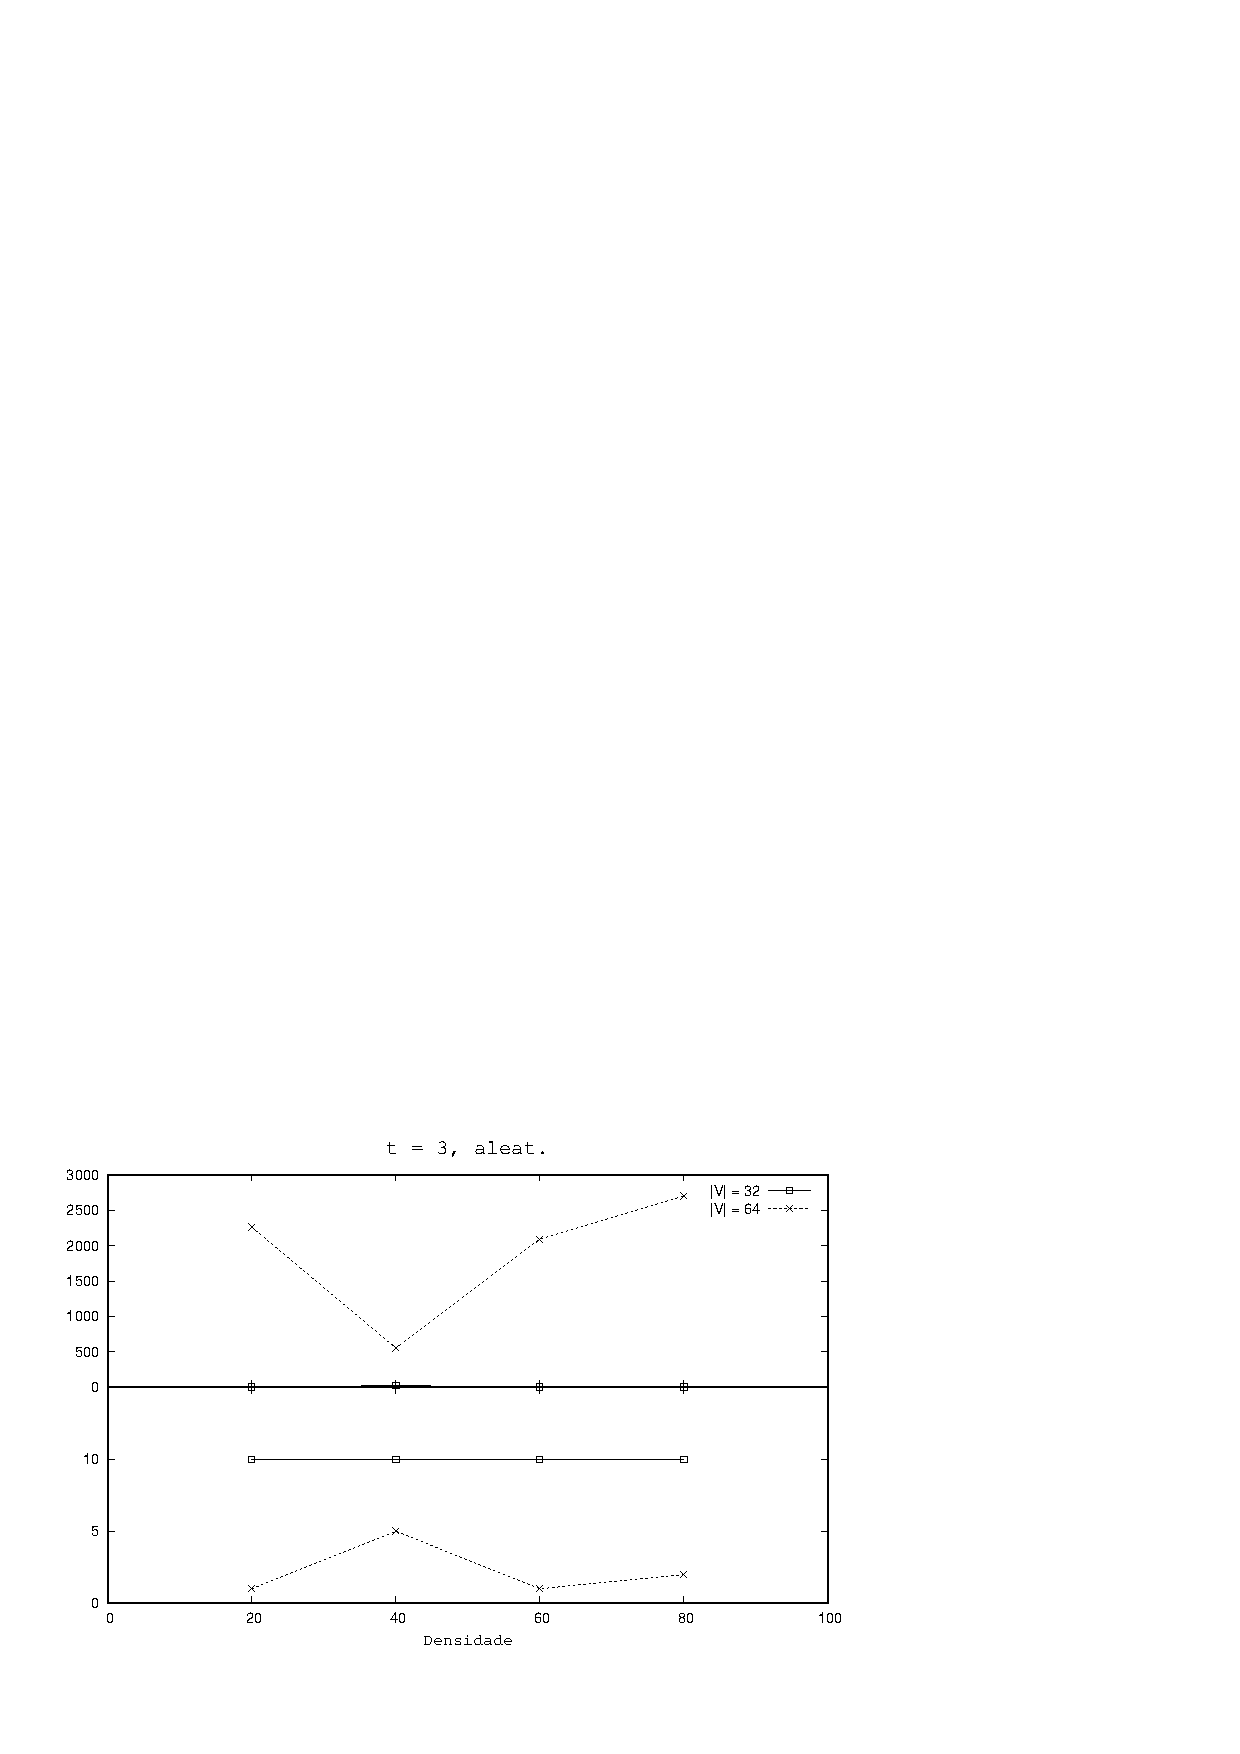
\includegraphics[scale=0.60]{figuras/time_inst_den-sf3-random} }}    
    %% \subfloat[label 2]{{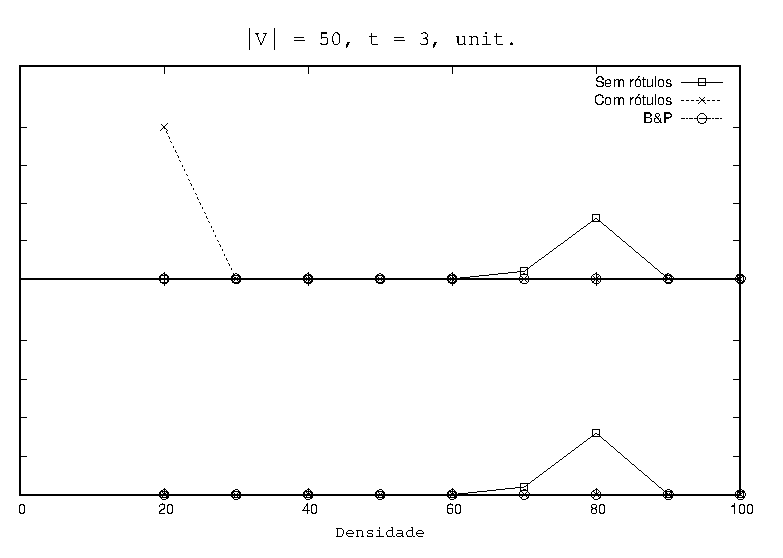
\includegraphics[scale=0.70]{figuras/2inst_den-sf3-s50-unit} }}%
    \caption{Tempo médio de execução e quantidade de instâncias resolvidas por B\&P para peso aleatório}%
    \label{fig:time_inst_den-sf2_sf3-random}%
\end{figure}

\begin{figure}[t]%
    \centering
    \subfloat{{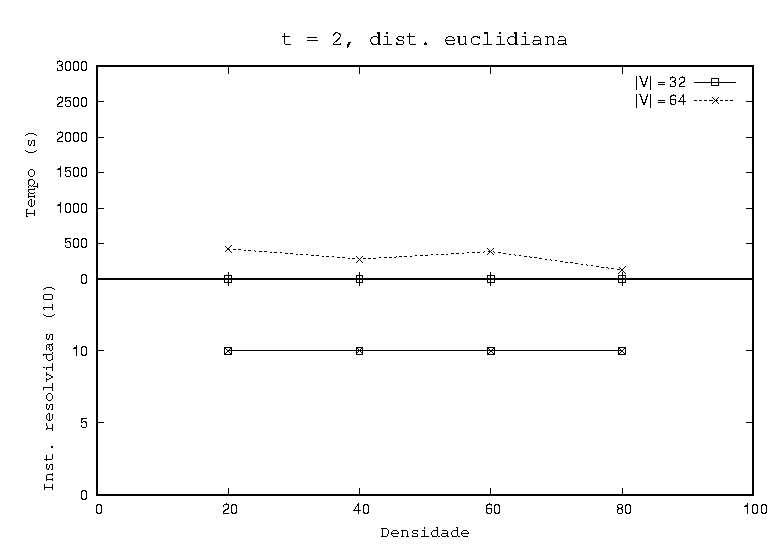
\includegraphics[scale=0.60]{figuras/time_inst_den-sf2-euclidean} }}%
    %\;
    \subfloat{{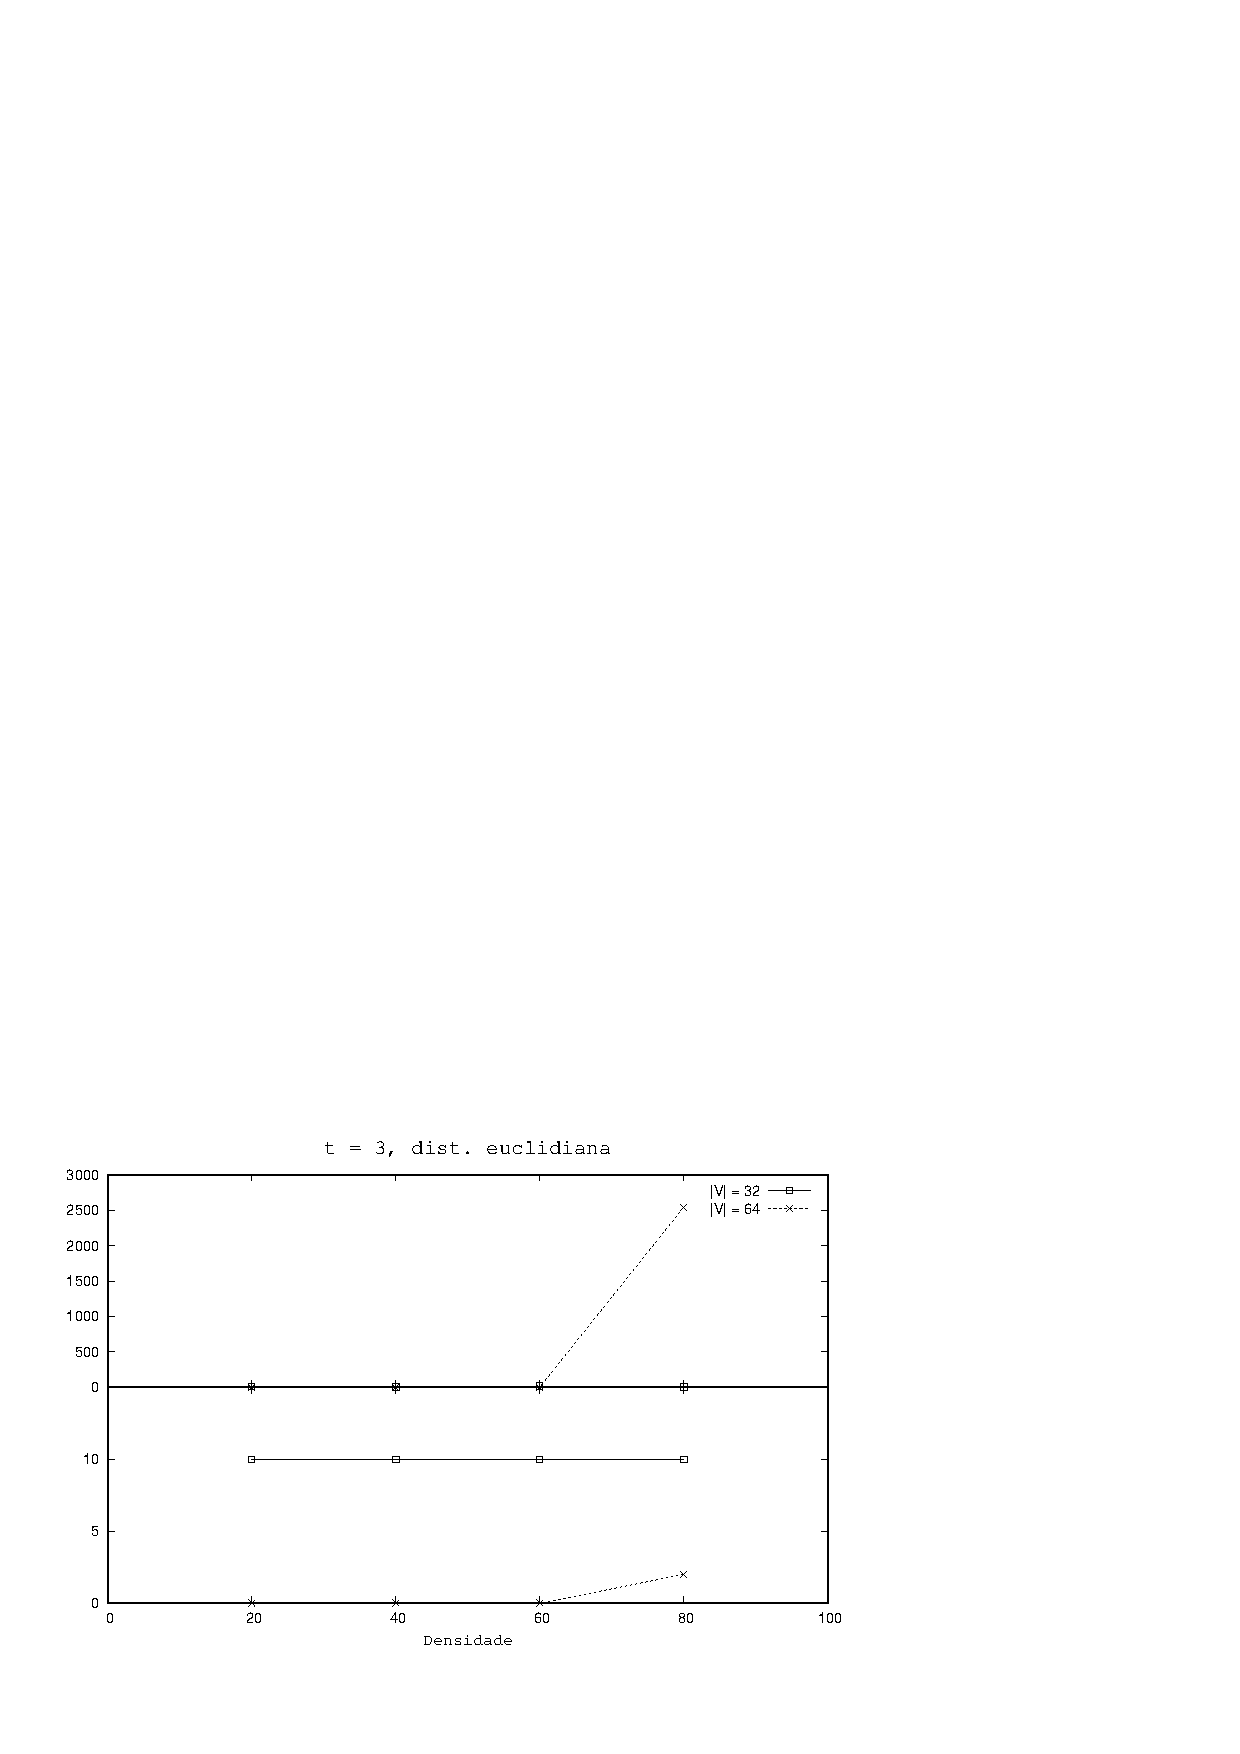
\includegraphics[scale=0.60]{figuras/time_inst_den-sf3-euclidean} }}    
    %% \subfloat[label 2]{{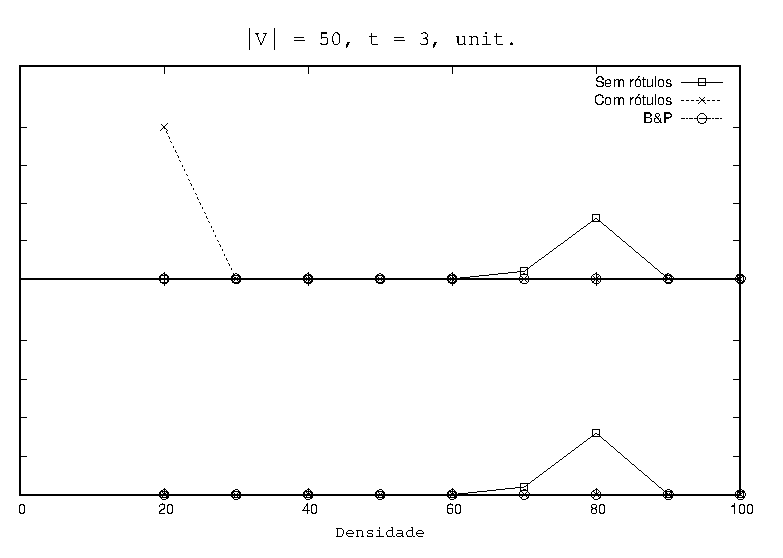
\includegraphics[scale=0.70]{figuras/2inst_den-sf3-s50-unit} }}%
    \caption{Tempo médio de execução e quantidade instâncias resolvidas por B\&P para distância euclidiana}%
    \label{fig:time_inst_den-sf2_sf3-euclidean}%
\end{figure}

%% \begin{center}
%%   \noindent
%%   \footnotesize{
%%     \begin{tabular}{|c|c|c|c|c|}\hline
%%       {Grau} & {$t$} & {Ordem} & {Média dos \emph{gaps} entre os limitantes (\%)} & {\# Instâncias}\\
%% \hline\hline      
%% 4	&	2	&	32	&	\num{0}	&	1	\\
%% 	&		&	64	&	\num{0,531}	&	3	\\
%% 	&	3	&	32	&	\num{3,42}	&	6	\\
%% 	&		&	64	&	\num{6,61}	&	10	\\
%% 	&	4	&	32	&	\num{2,44}	&	10	\\
%% 	&		&	64	&	\num{29,1}	&	10	\\
%% 8	&	2	&	16	&	\num{3,15}	&	8	\\
%% 	&		&	32	&	\num{7,69}	&	10	\\
%% 	&		&	64	&	\num{7,37}	&	10	\\
%% 	&	3	&	16	&	\num{6,67}	&	10	\\
%% 	&		&	32	&	\num{58,3}	&	10	\\
%% 	&		&	64	&	\num{83,3}	&	10	\\
%% 	&	4	&	32	&	\num{37,6}	&	10	\\
%% 	&		&	64	&	\num{74,8}	&	10	\\
%%       \hline\hline
%%     \end{tabular}      
%%   }
%% \captionof{table}{\emph{Gap} relativo entre os limitantes para peso unitário quando o grau é variado}\label{tab:gap_integralidade_unit_grau}  
%% \end{center}


%% Para as instâncias para as quais não foi possível resolver o MWSP
%% dentro do intervalo de tempo estabelecido, achamos que seria
%% interessante saber quão próximo a implementação estava de encontrar
%% uma solução ótima. Para isso, calculamos o \emph{intervalo (gap)
%%   relativo entre limitantes primal e dual}.


%%   Para um problema de minimização, o \emph{gap} relativo entre os limitantes
%%   em um determinado momento do algoritmo de B\&B consiste na
%%        diferença entre a melhor (menor) 
%%        solução inteira (solução incumbente) e a menor cota inferior
%%        (dentre todos os nós folhas da árvore de B\&B existentes neste momento) 
%%        para a função objetivo~\cite{Gurobi2019, Cplex2019}. Esta menor cota
%%        inferior também é conhecida como melhor cota inferior.
%%      No nosso caso, expressaremos essa diferença de maneira relativa, mais
%%      especificamente:
%%      \begin{align*}
%%        ((MelhorSolInteira - MelhorCotaInf) / MelhorCotaInf) * 100,
%%      \end{align*}
%%      onde \emph{MelhorSolInteira} corresponde à melhor solução inteira e
%%      \emph{MelhorCotaInf} corresponde à menor cota inferior para a função
%%      objetivo.

  
%%   %% Nós também verificamos o \emph{gap} de integralidade para cada
%%   %% instância para a qual não foi possível resolver o MWSP dentro do intervalo
%%   %% de tempo
%%   %% estabelecido. Nós queríamos saber quão próximo o resolvedor estava de
%%   %% encontrar uma solução ótima.
     
%%   Na Tabela~\ref{tab:gap_integralidade_unit_grau} mostramos 
%%   os \emph{gaps} entre os limitantes para o peso unitário, quando variamos o grau.
%%   A última coluna (\# Instâncias) mostra o número de instâncias que não puderam 
%%   ser resolvidas  dentro do intervalo de tempo estabelecido, mas para as quais 
%%   foi possível encontrar pelo menos uma solução viável. Na penúltima coluna,
%%   mostramos a média dos \emph{gaps} (levando em consideração
%%   a quantidade de instâncias da última coluna). 
%%   Pela Tabela~\ref{tab:gap_integralidade_unit_grau}, podemos ver que quanto
%%   maior
%%   o grau ou fator de dilatação ou ordem, pior o \emph{gap}.
%%   Para valores pequenos de fator de dilatação, podemos observar que o
%%   resolvedor quase encontrou uma solução ótima dentro do tempo estabelecido.
%%   Considerando as instâncias com peso nas arestas, para as instâncias
%%   as quais foi possível ser calculado o \emph{gap}, este se mostrou
%%   baixo, não passando de 11\%.
 

Vamos agora analisar o desempenho da implementação ao variar a densidade
dos grafos. Assim como quando o parâmetro variado era o  grau médio, as
instâncias com ambos os tipos de peso nas arestas são resolvidas rapidamente,
\sisetup{round-mode=places,round-precision=1}
mesmo para densidades altas, quando o fator de dilatação é $\num{1,1}$. Para os
\sisetup{round-mode=places,round-precision=0}
fatores de dilatação dois e três, as
Figura~\ref{fig:time_inst_den-sf2_sf3-random} e
Figura~\ref{fig:time_inst_den-sf2_sf3-euclidean} mostram o tempo
médio de execução e a quantidade de instâncias resolvidas no caso dos
pesos aleatórios e no caso das distâncias euclidianas,
respectivamente. Para o fator dois, no caso de quaisquer destes tipos de peso,
quase todas as instâncias são resolvidas.  Neste cenário, ao
considerarmos ordem~64, o tempo cresce consideravelmente quando comparado
à ordem~32. Para
fator três, ordem~64, e ambos os tipos de peso, ocorre uma queda considerável
(quando comparado à ordem~32) no
número de instâncias que podem ser resolvidas e um aumento substancial
no tempo de execução. Entre os dois tipos de peso, a implementação do B\&P tem
um desempenho melhor no caso de pesos aleatórios.

\begin{figure}%
    \centering
    \subfloat{{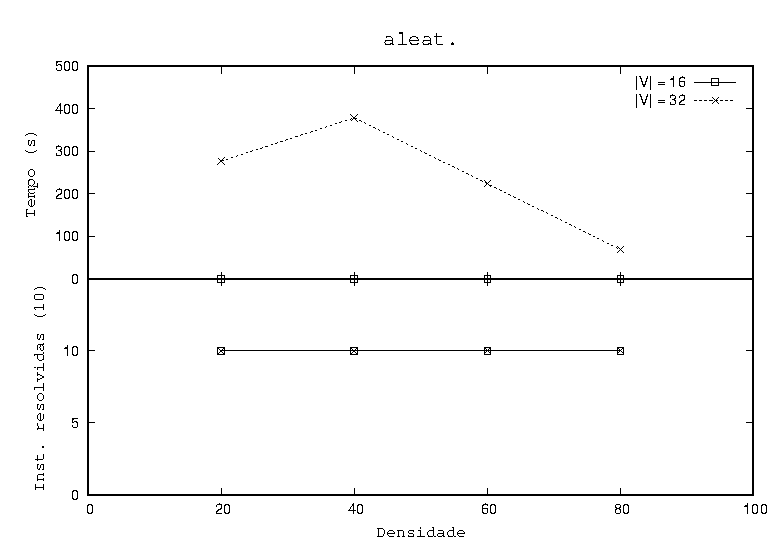
\includegraphics[scale=0.60]{figuras/time_inst_den-sf4-random} }}%
    %\;
    \subfloat{{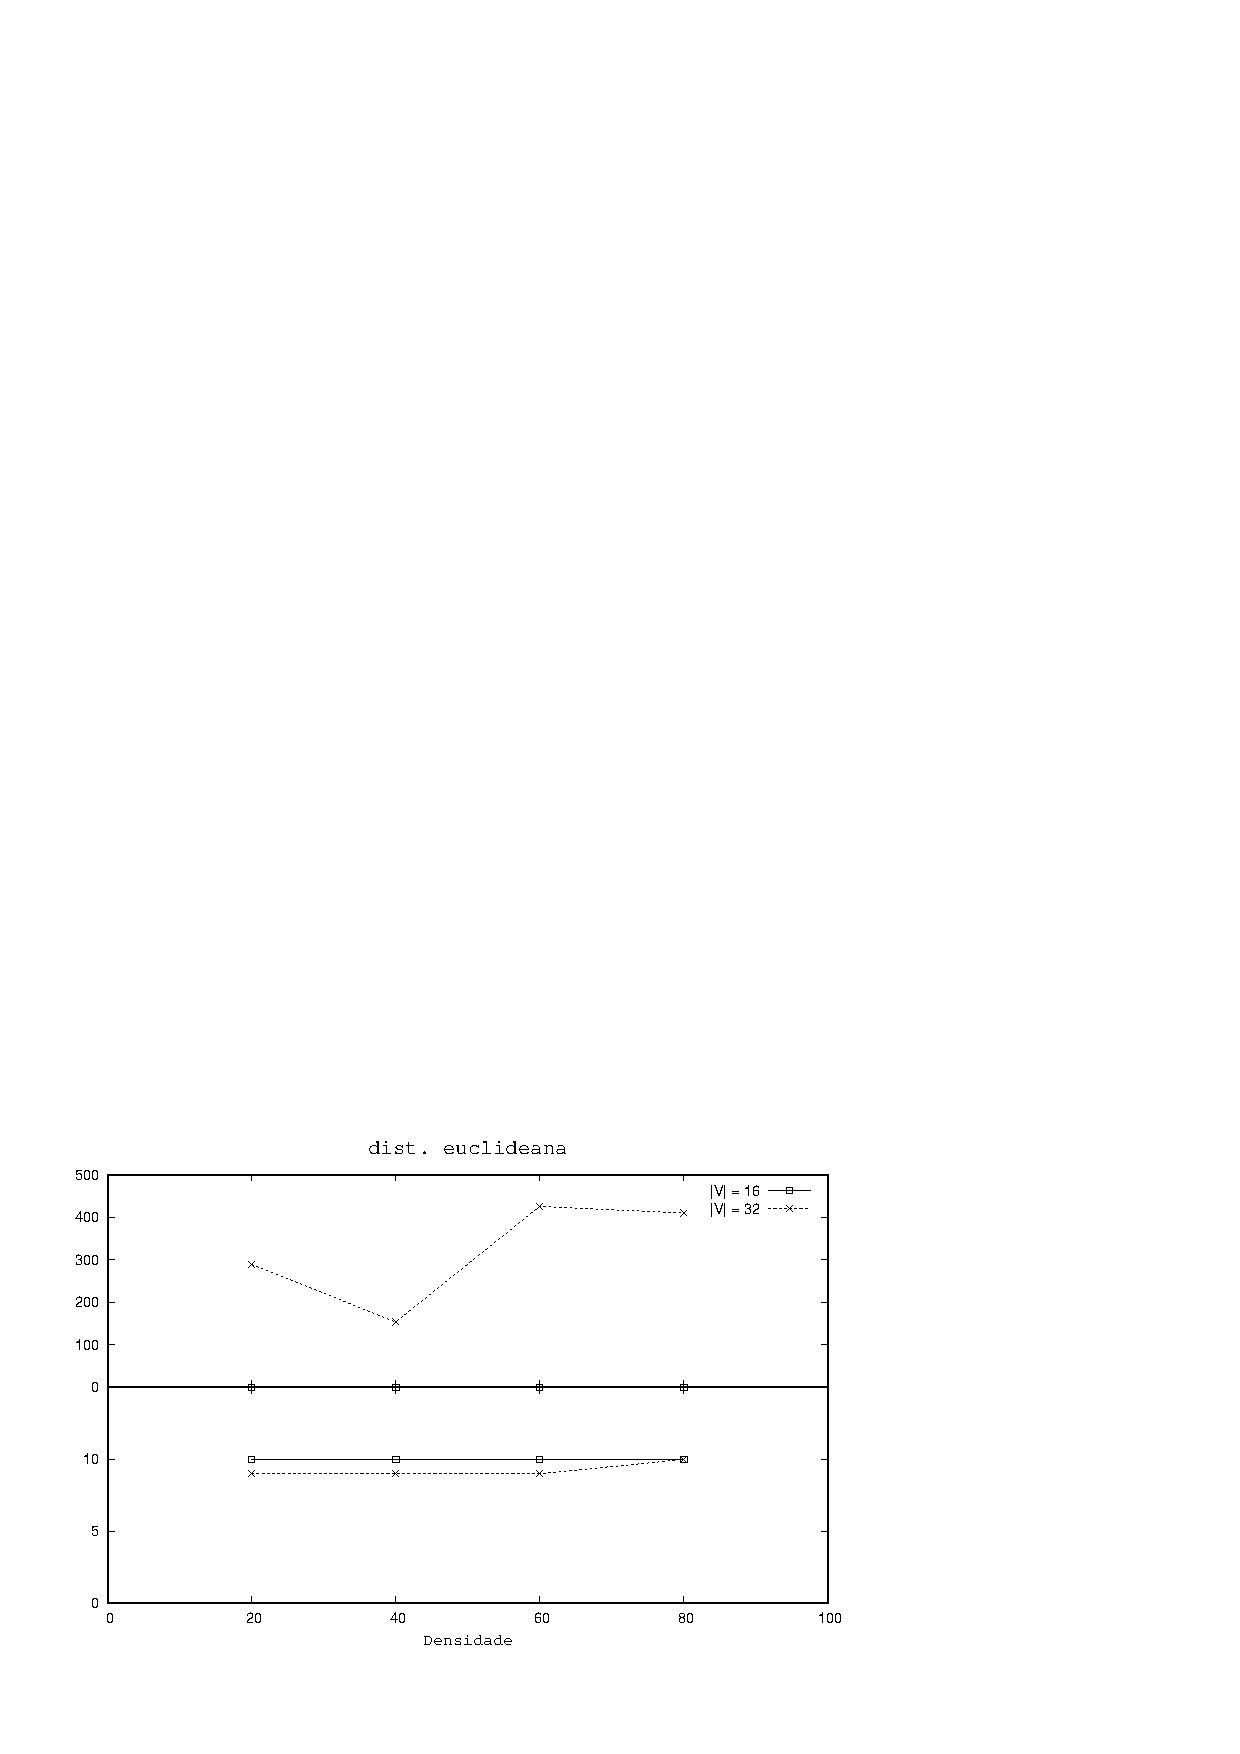
\includegraphics[scale=0.60]{figuras/time_inst_den-sf4-euclidean} }}    
    %% \subfloat[label 2]{{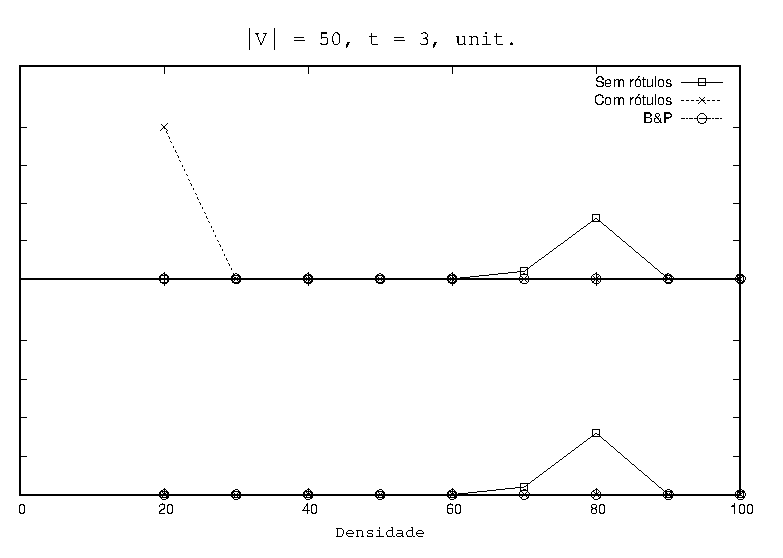
\includegraphics[scale=0.70]{figuras/2inst_den-sf3-s50-unit} }}%
    \caption{Tempo médio de execução e quantidade instâncias resolvidas por B\&P para $t = 4$ e arestas com peso}%
    \label{fig:time_inst_den-sf4-random_euclidean}%
\end{figure}

Ainda com relação aos grafos com ambos os pesos nas arestas, a
Figura~\ref{fig:time_inst_den-sf4-random_euclidean} mostra os
resultados para o fator de dilatação quatro. Resultados para grafos de
ordem~64 não são mostrados pois não foi possível resolver nenhuma
instância. Para ordens menores, assim como para os resultados
apresentados para $t = 3$, a implementação do B\&P é melhor quando o peso das
arestas é aleatório.

No caso dos pesos unitários, todas as instâncias são resolvidas
rapidamente quando a ordem do grafo é~16, exceto quando a densidade é
80\% (quando então o tempo de execução cresce consideravelmente). Para
$t = 2$, a implementação consegue resolver algumas instâncias de ordem~32,
mas com um tempo bastante alto. Todavia, não resolve nenhuma instância
de ordem~64. Para valores maiores de fator de dilatação, nenhuma
instância é resolvida quando a ordem é pelo menos~32.

%% \begin{center}
%%   \noindent
%%   \footnotesize{
%%     \begin{tabular}{|c|c|c|c|c|}\hline
%%       {$t$} & {Dens.} & {Ordem} & {Média dos \emph{gaps} entre limitantes (\%)} & {\# Instâncias}\\
%%       \hline\hline
%% 2	&	20	&	32	&	\num{2,82}	&	7	\\
%% 	&	40	&		&	\num{1,21}	&	9	\\
%% 	&	20	&	64	&	\num{36}	&	10	\\
%% 	&	40	&		&	\num{38,4}	&	10	\\
%% 	&	60	&		&	\num{36,9}	&	10	\\
%% 	&	80	&		&	\num{36,9}	&	10	\\
%% 3	&	20	&	32	&	\num{41}	&	10	\\
%% 	&	40	&		&	\num{39,3}	&	10	\\
%% 	&	60	&		&	\num{25,3}	&	10	\\
%% 	&	80	&		&	\num{28,4}	&	10	\\
%% 	&	20	&	64	&	\num{155}	&	5	\\
%% 	&	40	&		&	\num{265}	&	2	\\
%% 	&	60	&		&	\num{159}	&	5	\\
%% 	&	80	&		&	\num{154}	&	7	\\
%%       \hline\hline
%%     \end{tabular}      
%%   }
%% \captionof{table}{\emph{Gap} relativo entre limitantes para peso unitário quando a densidade é variada}\label{tab:gap_integralidade_unit_dens}  
%% \end{center}


%% \begin{center}
%%   \noindent
%%   \footnotesize{
%%     \begin{tabular}{|c|c|c|c|c|}\hline
%%       {$t$} & {Dens.} & {Ordem} & {Média do \emph{gap} entre limitantes (\%)} & {\# Instâncias}\\
%%       \hline\hline
%% 3	&	20	&	64	&	\num{1,38}	&	7	\\
%% 	&	40	&		&	\num{14,6}	&	4	\\
%% 	&	60	&		&	\num{3,42}	&	7	\\
%% 	&	80	&		&	\num{1,3}	&	4	\\
%% 4	&	20	&		&	\num{22,9}	&	7	\\
%% 	&	40	&		&	\num{17,5}	&	10	\\
%% 	&	60	&		&	\num{11,5}	&	10	\\
%% 	&	80	&		&	\num{15,5}	&	10	\\
%%       \hline\hline
%%     \end{tabular}      
%%   }
%% \captionof{table}{\emph{Gap} relativo entre limitantes para peso aleatório quando a densidade é variada}\label{tab:gap_integralidade_random_dens}  
%% \end{center}


%% Nós também verificamos os \emph{gaps} entre limitantes quando o
%% parâmetro variado é a densidade. As
%% Tabelas~\ref{tab:gap_integralidade_unit_dens} e
%% \ref{tab:gap_integralidade_random_dens} mostram os valores do
%% \emph{gap} para peso aleatório e peso unitário, respectivamente.
%% Podemos ver que, para peso aleatório, os valores do \emph{gap} são bem
%% menores quando comparados aos valores para o peso unitário.
%%   %% Para este cenário, mesmo para ordem~32, quando o fator de dilatação é três,
%%   %% os \emph{gaps} são muito altos. Podemos inferir que mesmo aumentando um
%%   %% pouco o tempo de limite para resolver cada instância, provavelmente não
%%   %% será suficiente. Para as instâncias com peso nas arestas, os \emph{gaps}
%%   %% também não foram baixos. 


Quando o fator de dilatação é grande (pelo menos três) e/ou a
densidade é grande, em geral, o número de soluções viáveis
($t$-spanners) cresce muito, exigindo um tempo de execução bem
grande. Os diversos testes computacionais dão ao leitor uma indicação de
tipos de
instâncias que a implementação do B\&P pode resolver. Mas, é difícil
prever como será o desempenho da implementação em instâncias que não
são do tipo que consideramos. Em breve, deixaremos disponível na
internet os códigos de nossa implementação para que os interessadas
possam fazer uso. 
